
\chapter{Results}

The algorithms have been evaluated with 1120 mono sounds from the test dataset for the Kaggle Audio tagging competition created by the MTG and Freesound. The test set for the dataset is an accurate representation of the content of the whole dataset for the competition. The dataset has been manually anotated by the author using the script evaluation.py in the Evaluation folder on thew github repository. The evaluation was carried by annotating the existance of the following problems: Hum, Clicks, Noise Bursts, Saturation and Silence. Other algorithms that had to be evaluated were Phase issues. However, as the dataset is formed exclusively of mono files, the algorithms were not properly evaluated.

The parameter values evaluated for each algorithms will be evaluated with 3 measures: precision \ref{eqn:precision}, recall \ref{eqn:recall} and $F_{0.5}$ score \ref{eqn:FScore}. A value of $\beta=0.5$ was chosen to weight the score in favor of the precision score.

\begin{equation}\label{eqn:precision}
	Precision = \frac{TruePositive}{TruePositive + FalsePositive}
\end{equation}
\begin{equation}\label{eqn:recall}
	Recall = \frac{TruePositive}{TruePositive + FalseNegative}
\end{equation}
\begin{equation}\label{eqn:FScore}
	F_{\beta} = (1+\beta^2)\frac{precision \cdot recall}{\beta^2 \cdot precision + recall}, F_{0.5} = 1.25\frac{precision \cdot recall}{0.25 \cdot precision + recall}
\end{equation}

\section{Hum detection evaluation}
Four parameters of the essentia Hum algorithm were considered in the evaluation: TimeWindow, minimumDuration, NumberofHarmonics and timeContinuity. The timeWindow parameter is a measure of the analysis time to use in the Hum estimation in s. The parameter was evaluated for the values: [0.1, 0.3, 0.5, 1, 3, 5] as they seemed a good sweep of values for the parameter. However, as it can be seen in the results obtained in \ref{fig:humTimeWindow}, they are not satisfactory, as the values remain constant at 0 and 1 which, inspecting the equations and knowing that a 0/0 indetermination will be considered with a value of 1 as a result, can be extrapolated that: a recall score of 0 means a TruePositive count of 0, and then, a precision value of 1 with a TruePositive count of 0 means that the denominator also is 0 and we can conclude that FalsePositive values are also 0 which means that all audio files were detected as Healthy and by manual revision it can be seen that there are audio files that have hum so this parameter is not relevant to the detection.

\begin{figure}[H]
	\centering
	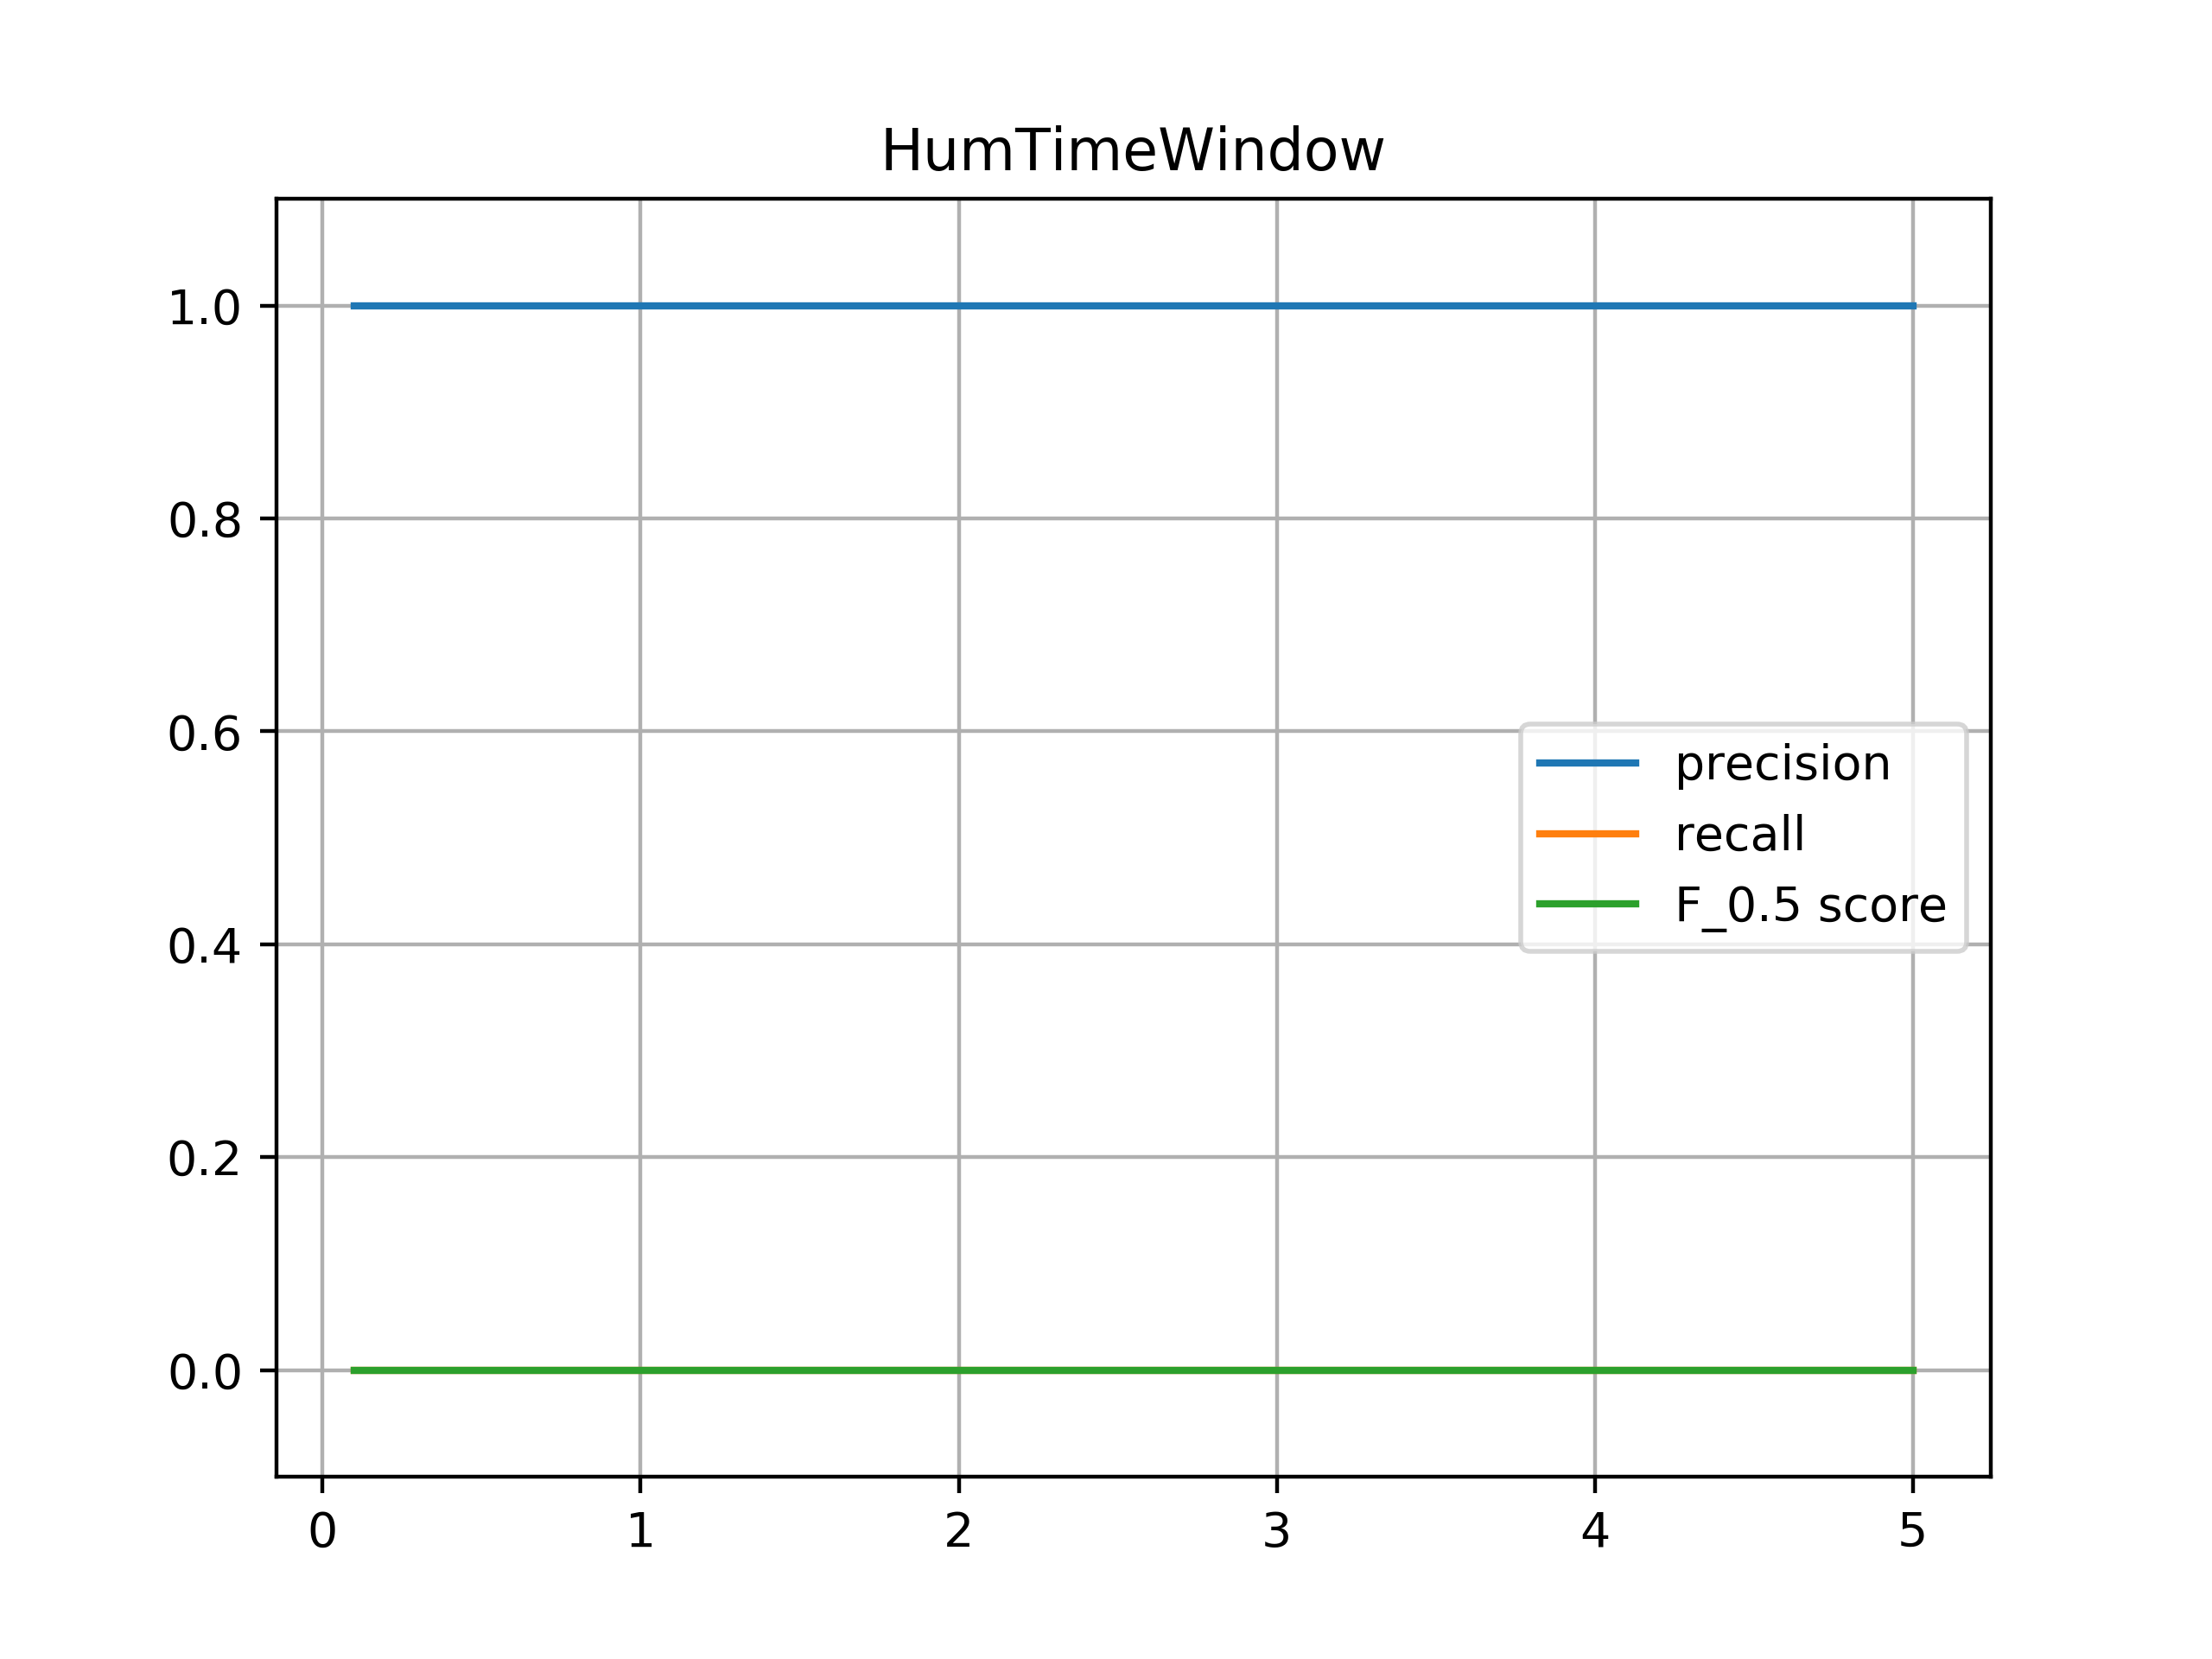
\includegraphics[clip, width=0.7\columnwidth]{Figures/HumTimeWindow.png}% 
	\caption{timeWindow parameter sweep results (accuracy, F score and recall)}
	\label{fig:humTimeWindow}
\end{figure}

The next parameter to be evaluated is minimumDuration, which is the minimum time span for which the hum is detected. The parameter was sweeped through the range: [0.01, 0.07, 0.1, 0.3, 0.5, 1, 3, 5]. However, similar results to the previous ones were obtained, as can be seen in \ref{fig:humminimumDuration}.

\begin{figure}[H]
	\centering
	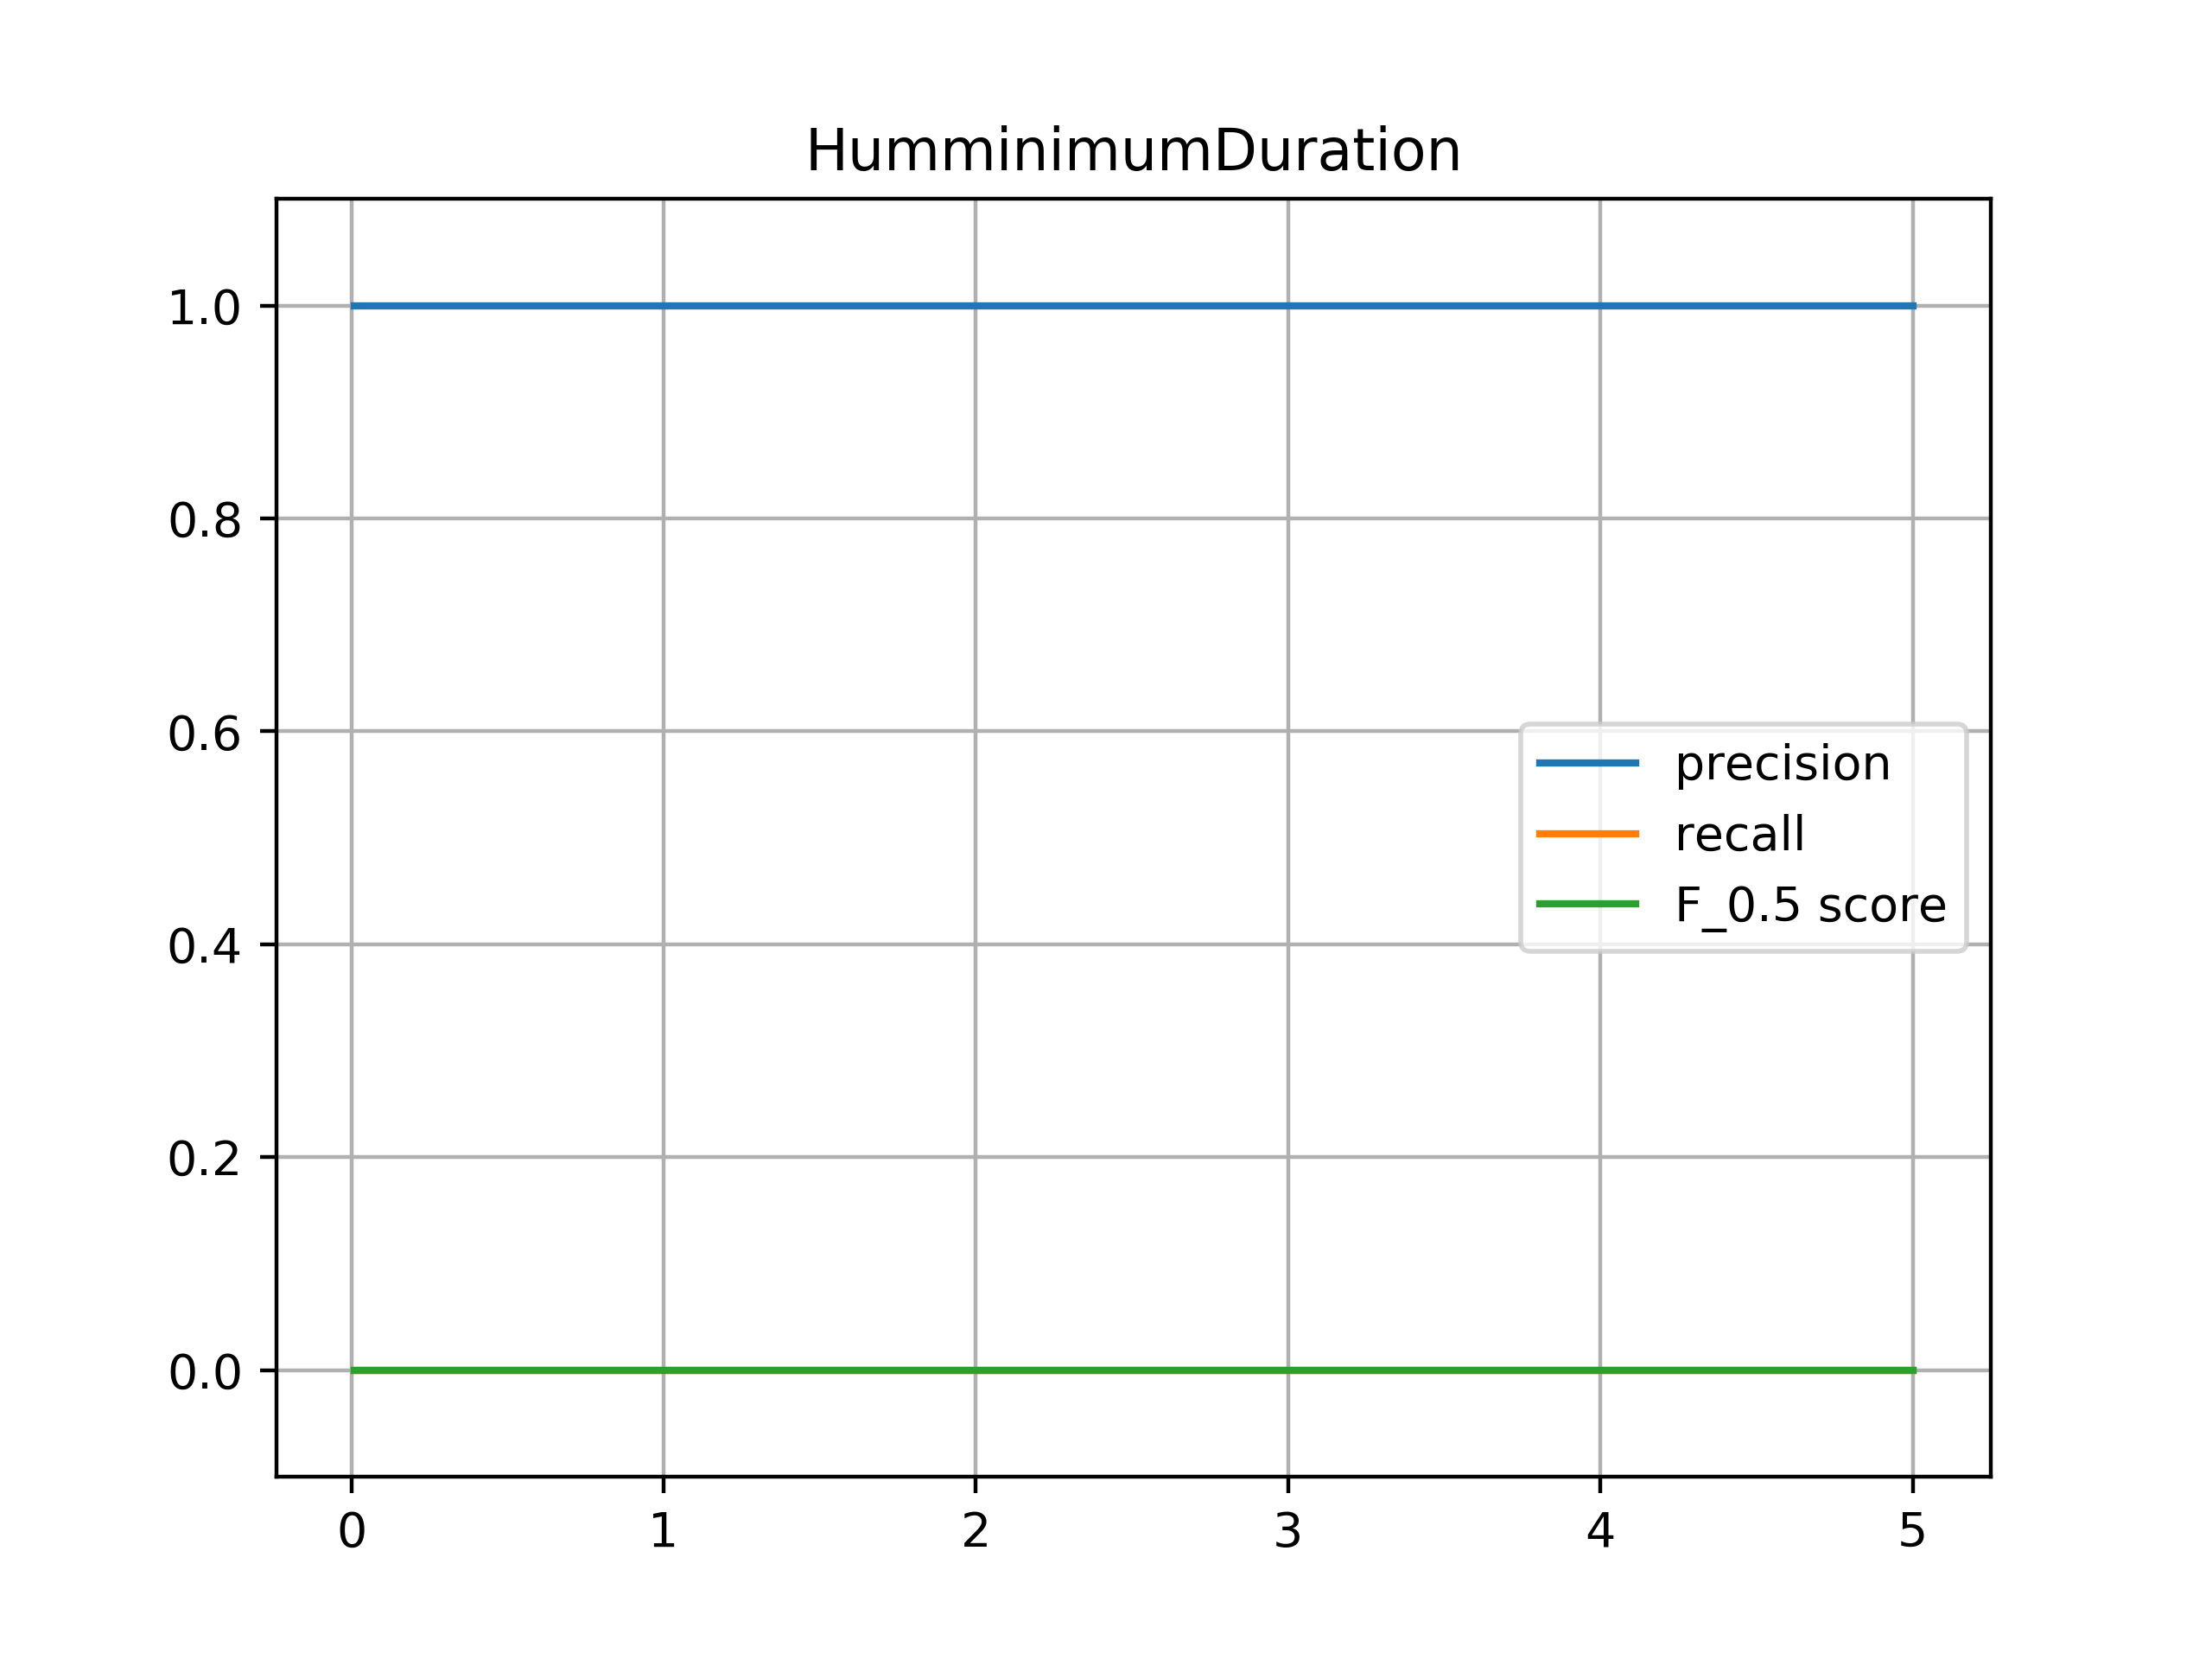
\includegraphics[clip,width=0.7\columnwidth]{Figures/HumminimumDuration.png}% 
	\caption{minimumDuration parameter sweep results (accuracy, F score and recall)}
	\label{fig:humminimumDuration}
\end{figure}

The next parameter to be evaluated is NumberofHarmonics, number of harmonic components for which the algorithm will look for it to consider a humming frequency. The parameter was sweeped through the range: [1, 2, 3, 4, 5]. However, similar results to the previous ones were obtained, as can be seen in \ref{fig:humnumberHarmonics}.

\begin{figure}[H]
	\centering
	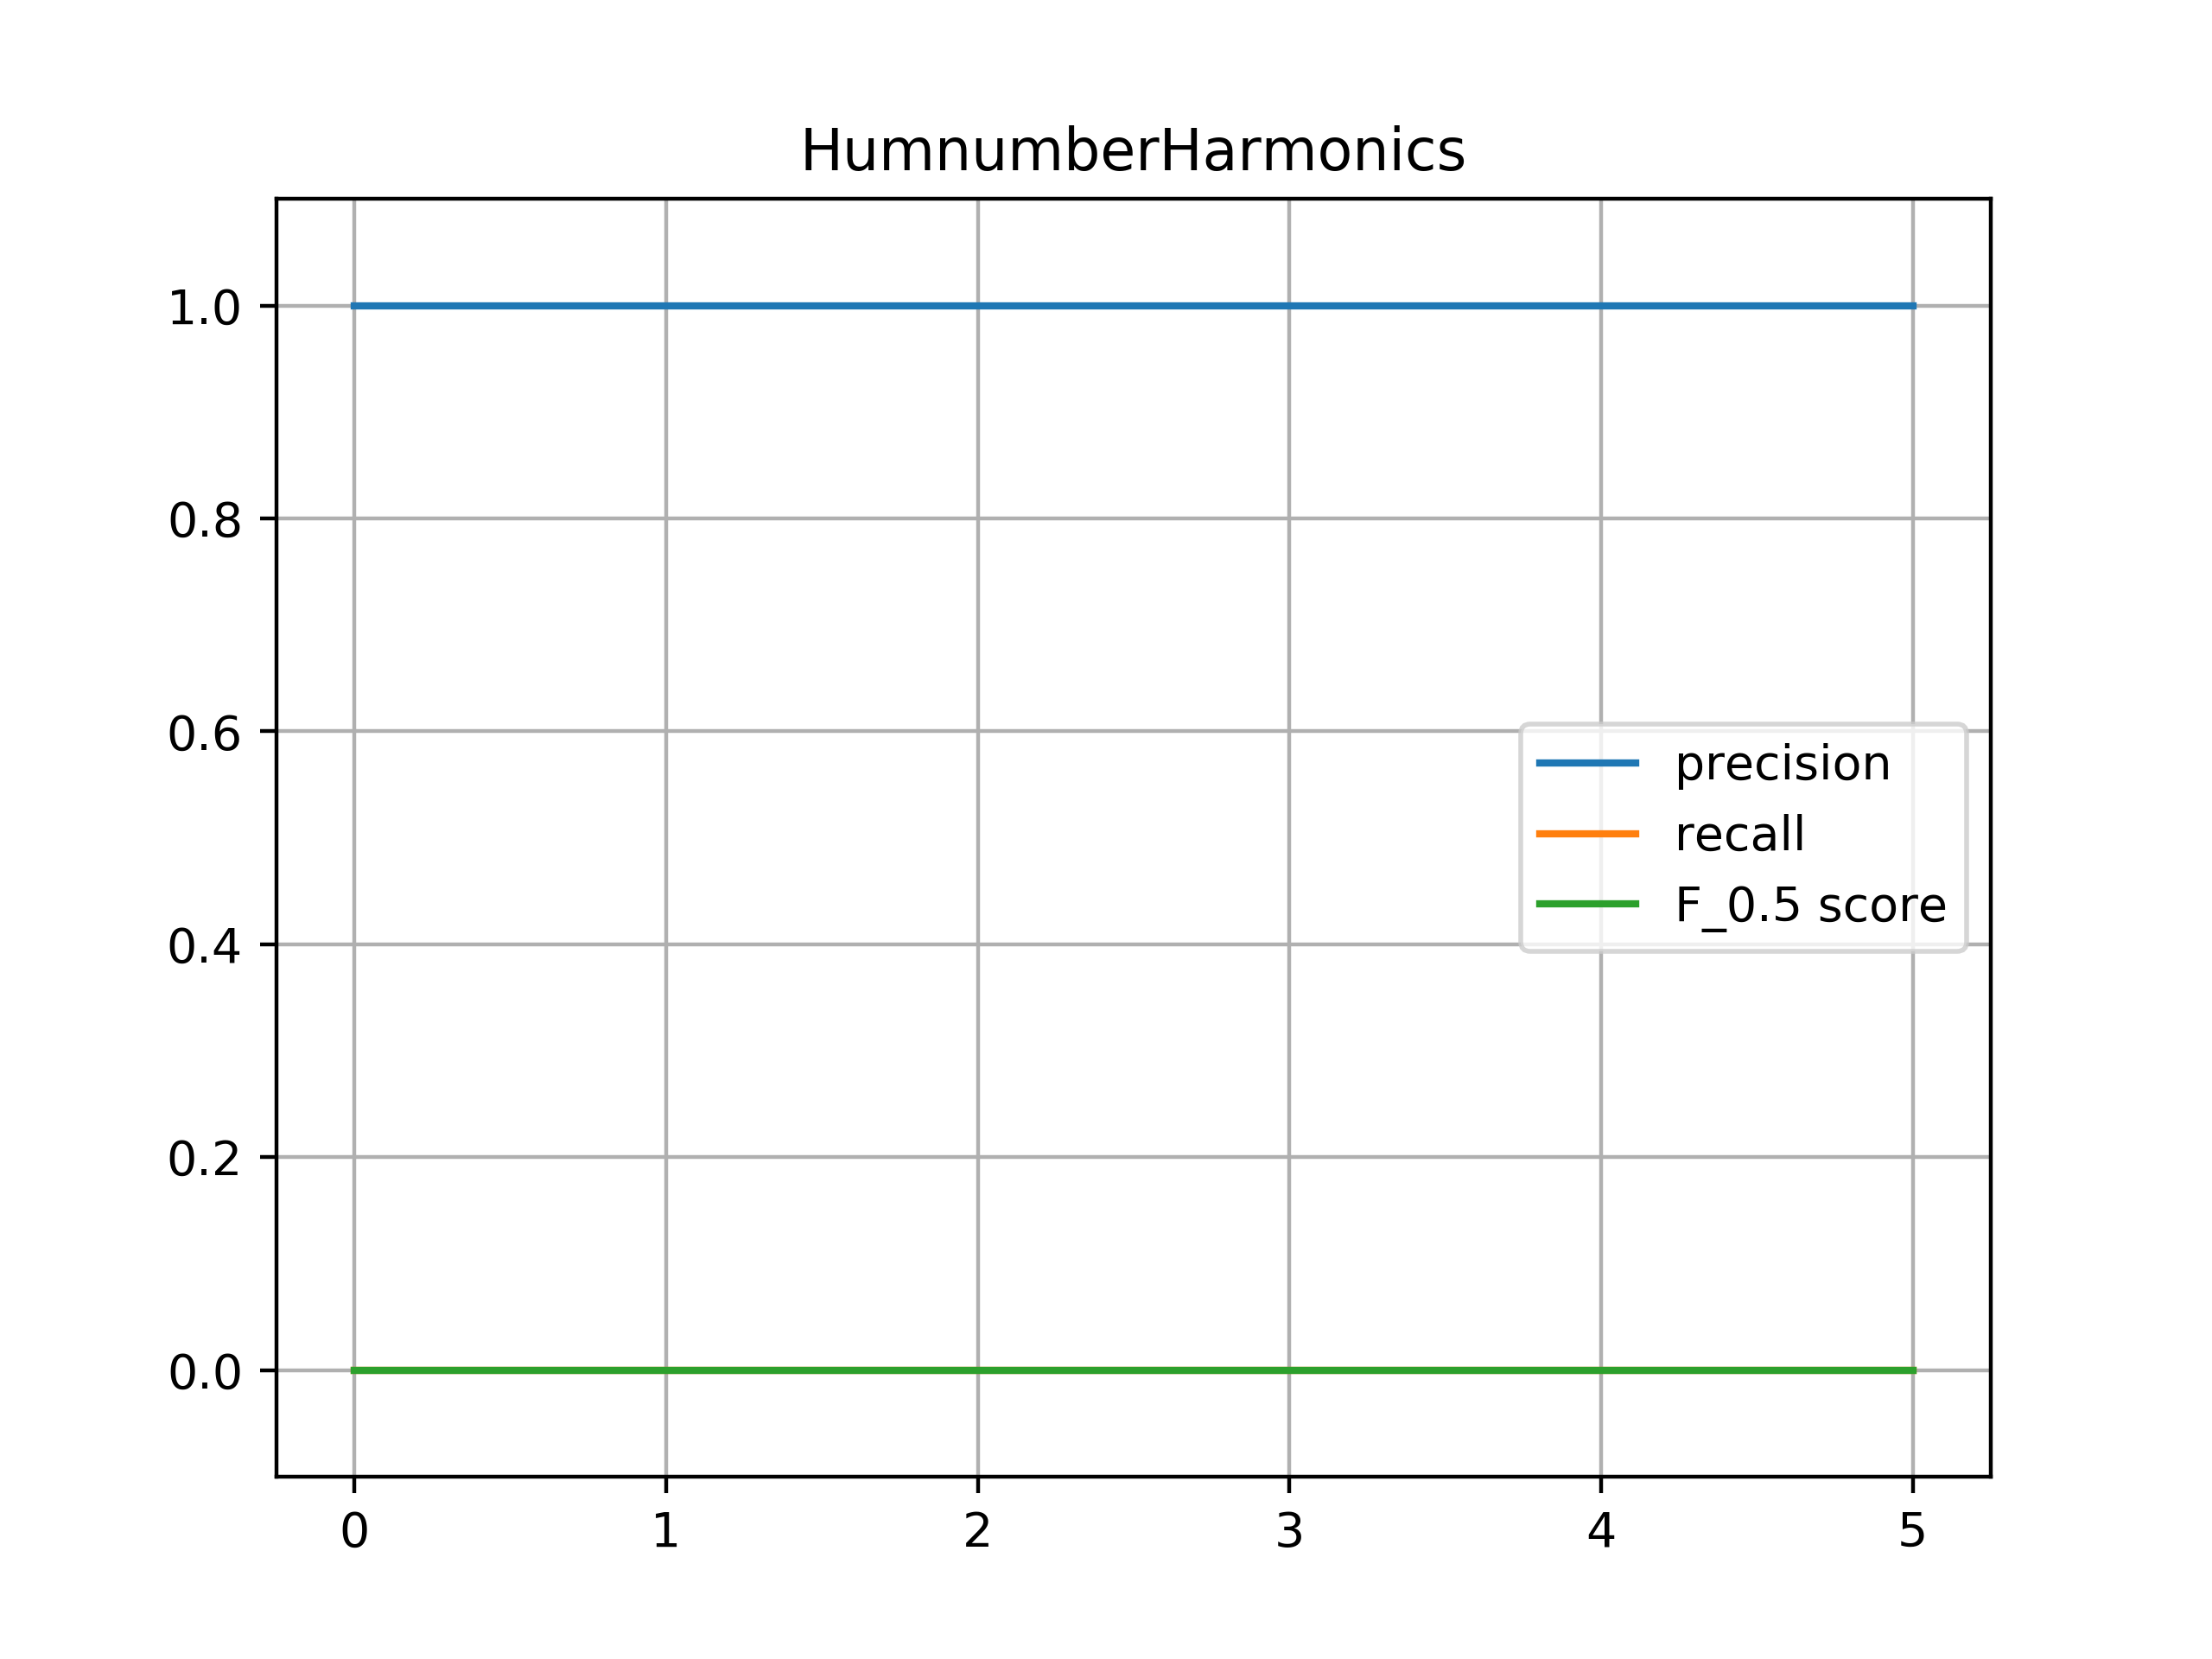
\includegraphics[clip,width=0.7\columnwidth]{Figures/HumnumberHarmonics.png}% 
	\caption{numberHarmonics parameter sweep results (accuracy, F score and recall)}
	\label{fig:humnumberHarmonics}
\end{figure}

The next parameter to be evaluated is timeContinuity, the minimum time for a humming frequency to be present to be detected. The parameter was sweeped through the range: [0.1, 0.3, 0.5, 1, 3, 5]. However, similar results to the previous ones were obtained, as can be seen in \ref{fig:humtimeContinuity}.

\begin{figure}[H]
	\centering
	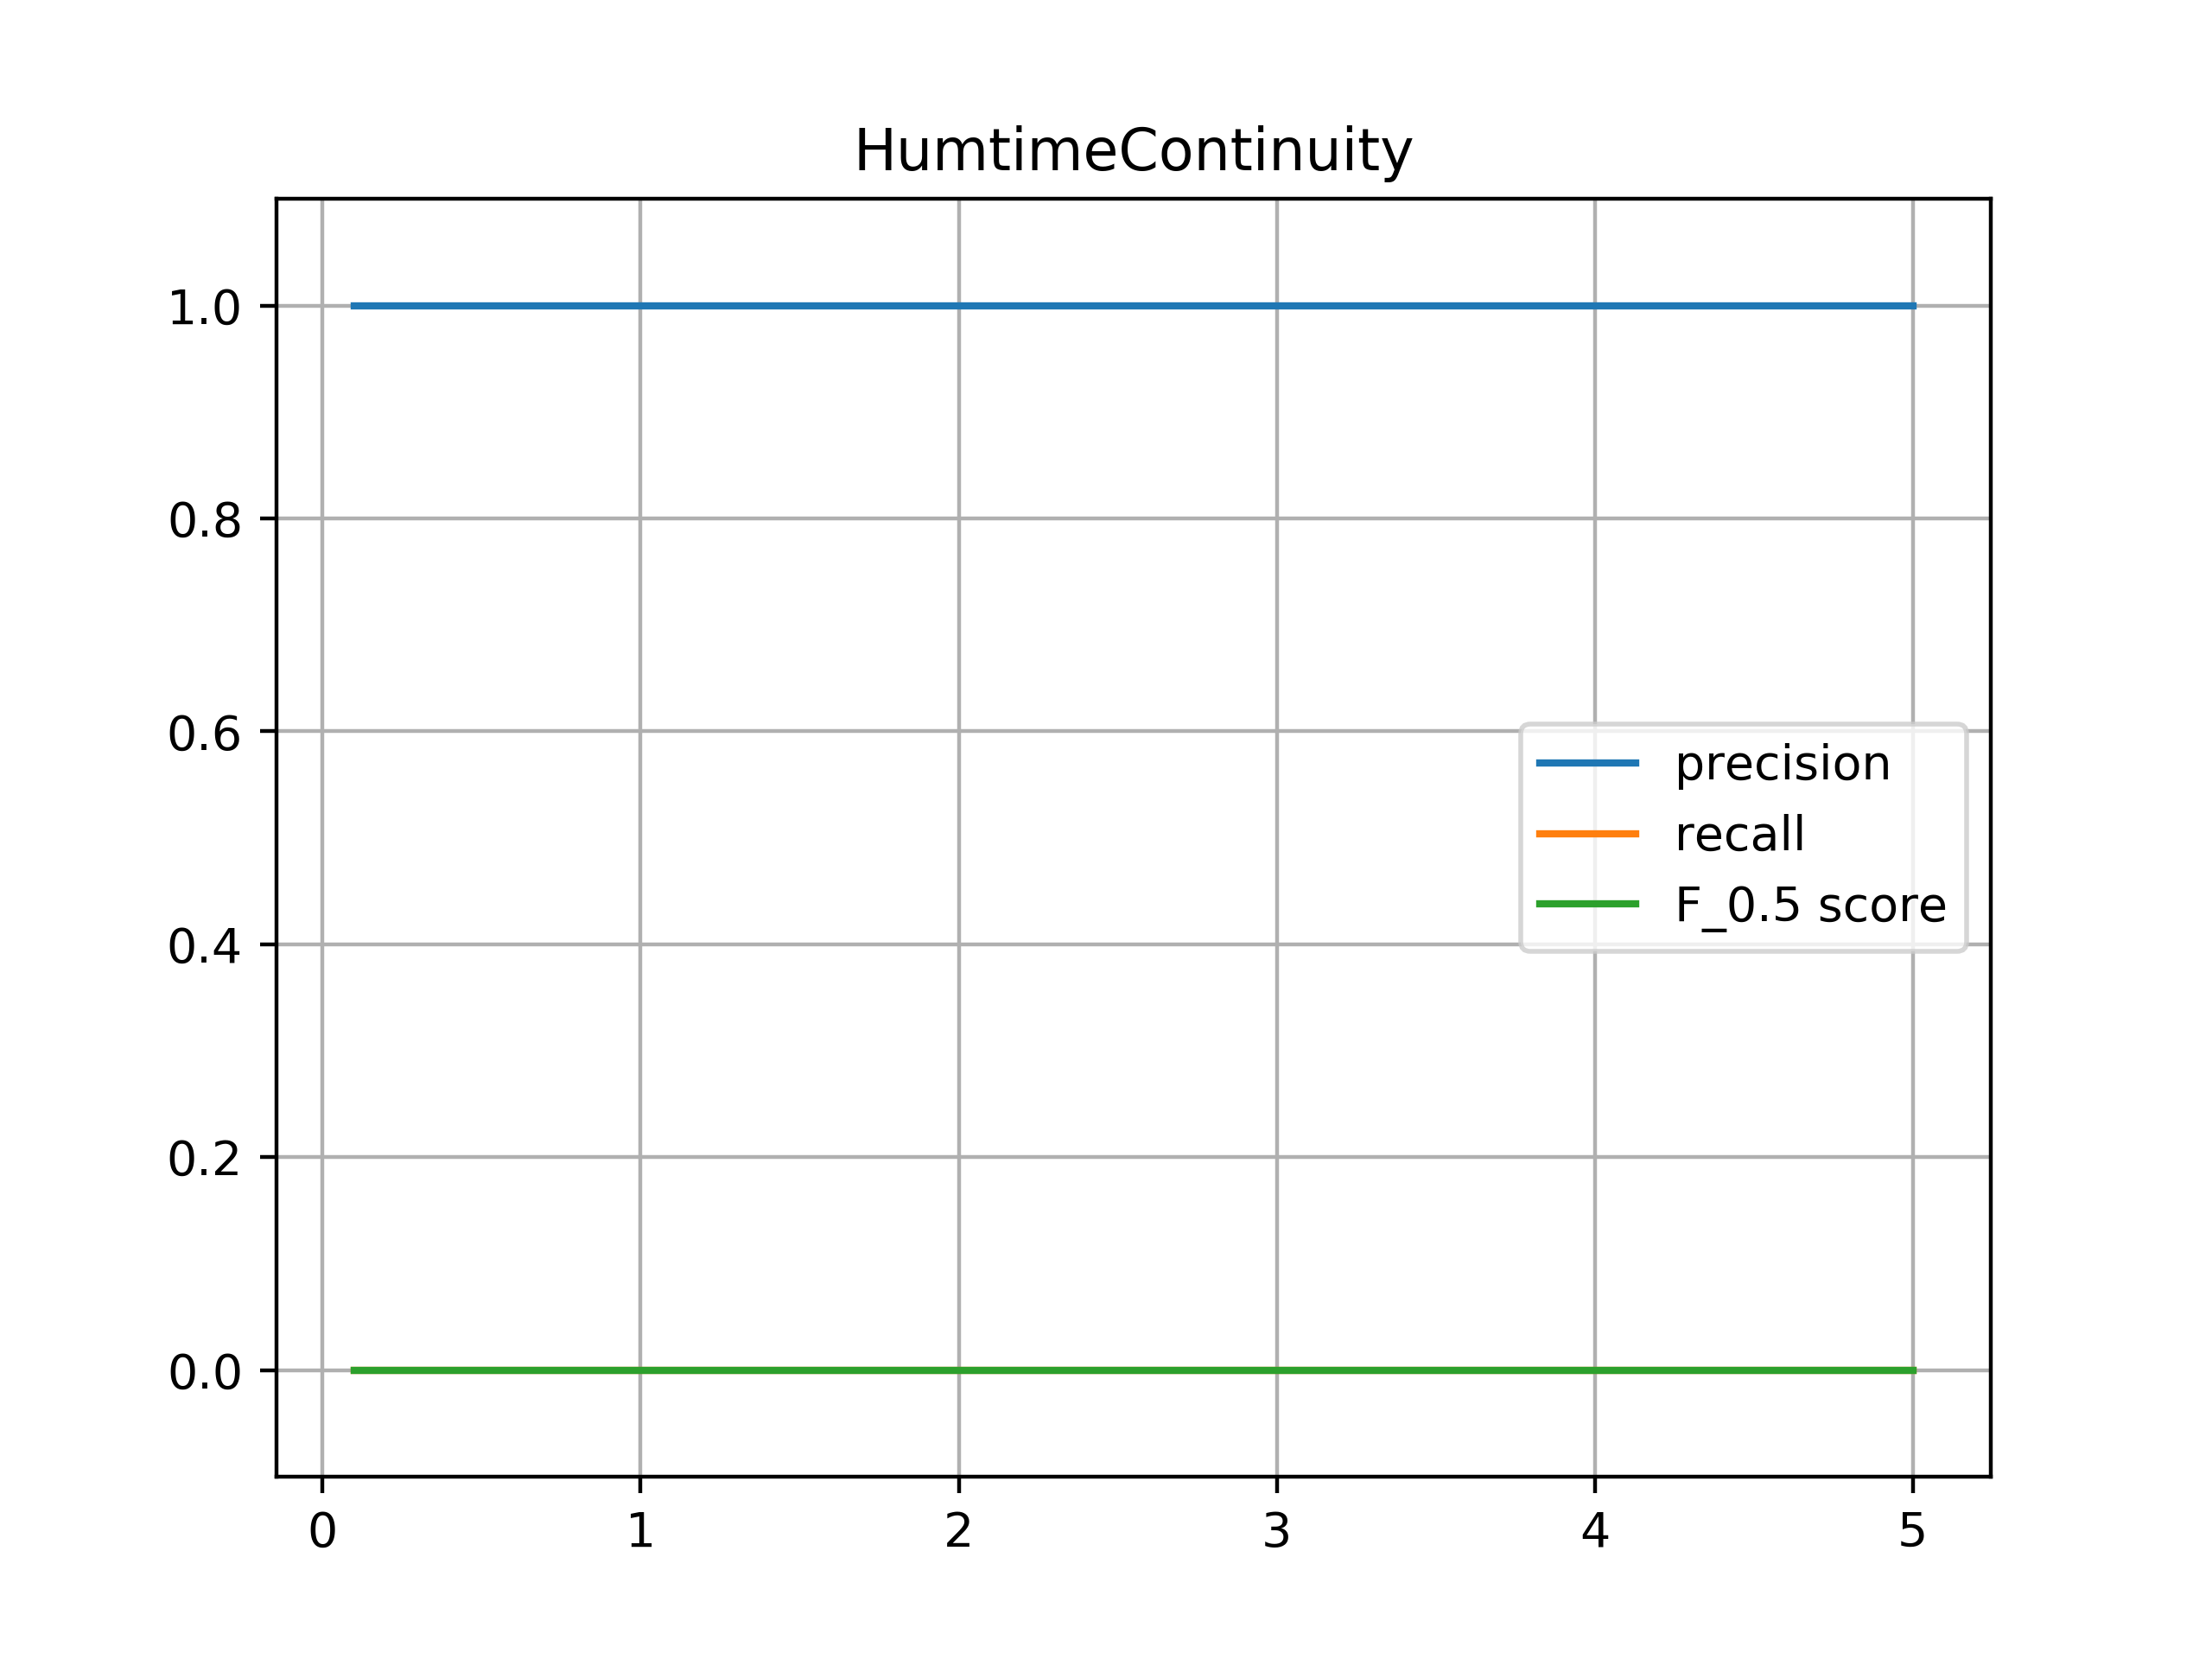
\includegraphics[clip,width=0.7\columnwidth]{Figures/HumtimeContinuity.png}% 
	\caption{timeContinuity parameter sweep results (accuracy, F score and recall)}
	\label{fig:humtimeContinuity}
\end{figure}

\section{Clicks detection evaluation}
Four parameters for the essentia clicks detector algorithm were evaluated: detectionThreshold, order, powerEstimationThreshold, silenceThreshold. The first parameter is detectionThreshold, which is based on the instant power of the noisy excitation signal plus detectionThreshold dBs. detectionThreshold parameter was swept in the range of values: [0, 5, 10, 15, 20, 25, 30, 35]. The results are as seen in \ref{fig:clicksdetectionThreshold}. As seen in the figure, the best results (maximum of the Fscore result) were obtained for a value of 25dB and the obtained Fscore obtained is about a 0.35.

\begin{figure}[H]
	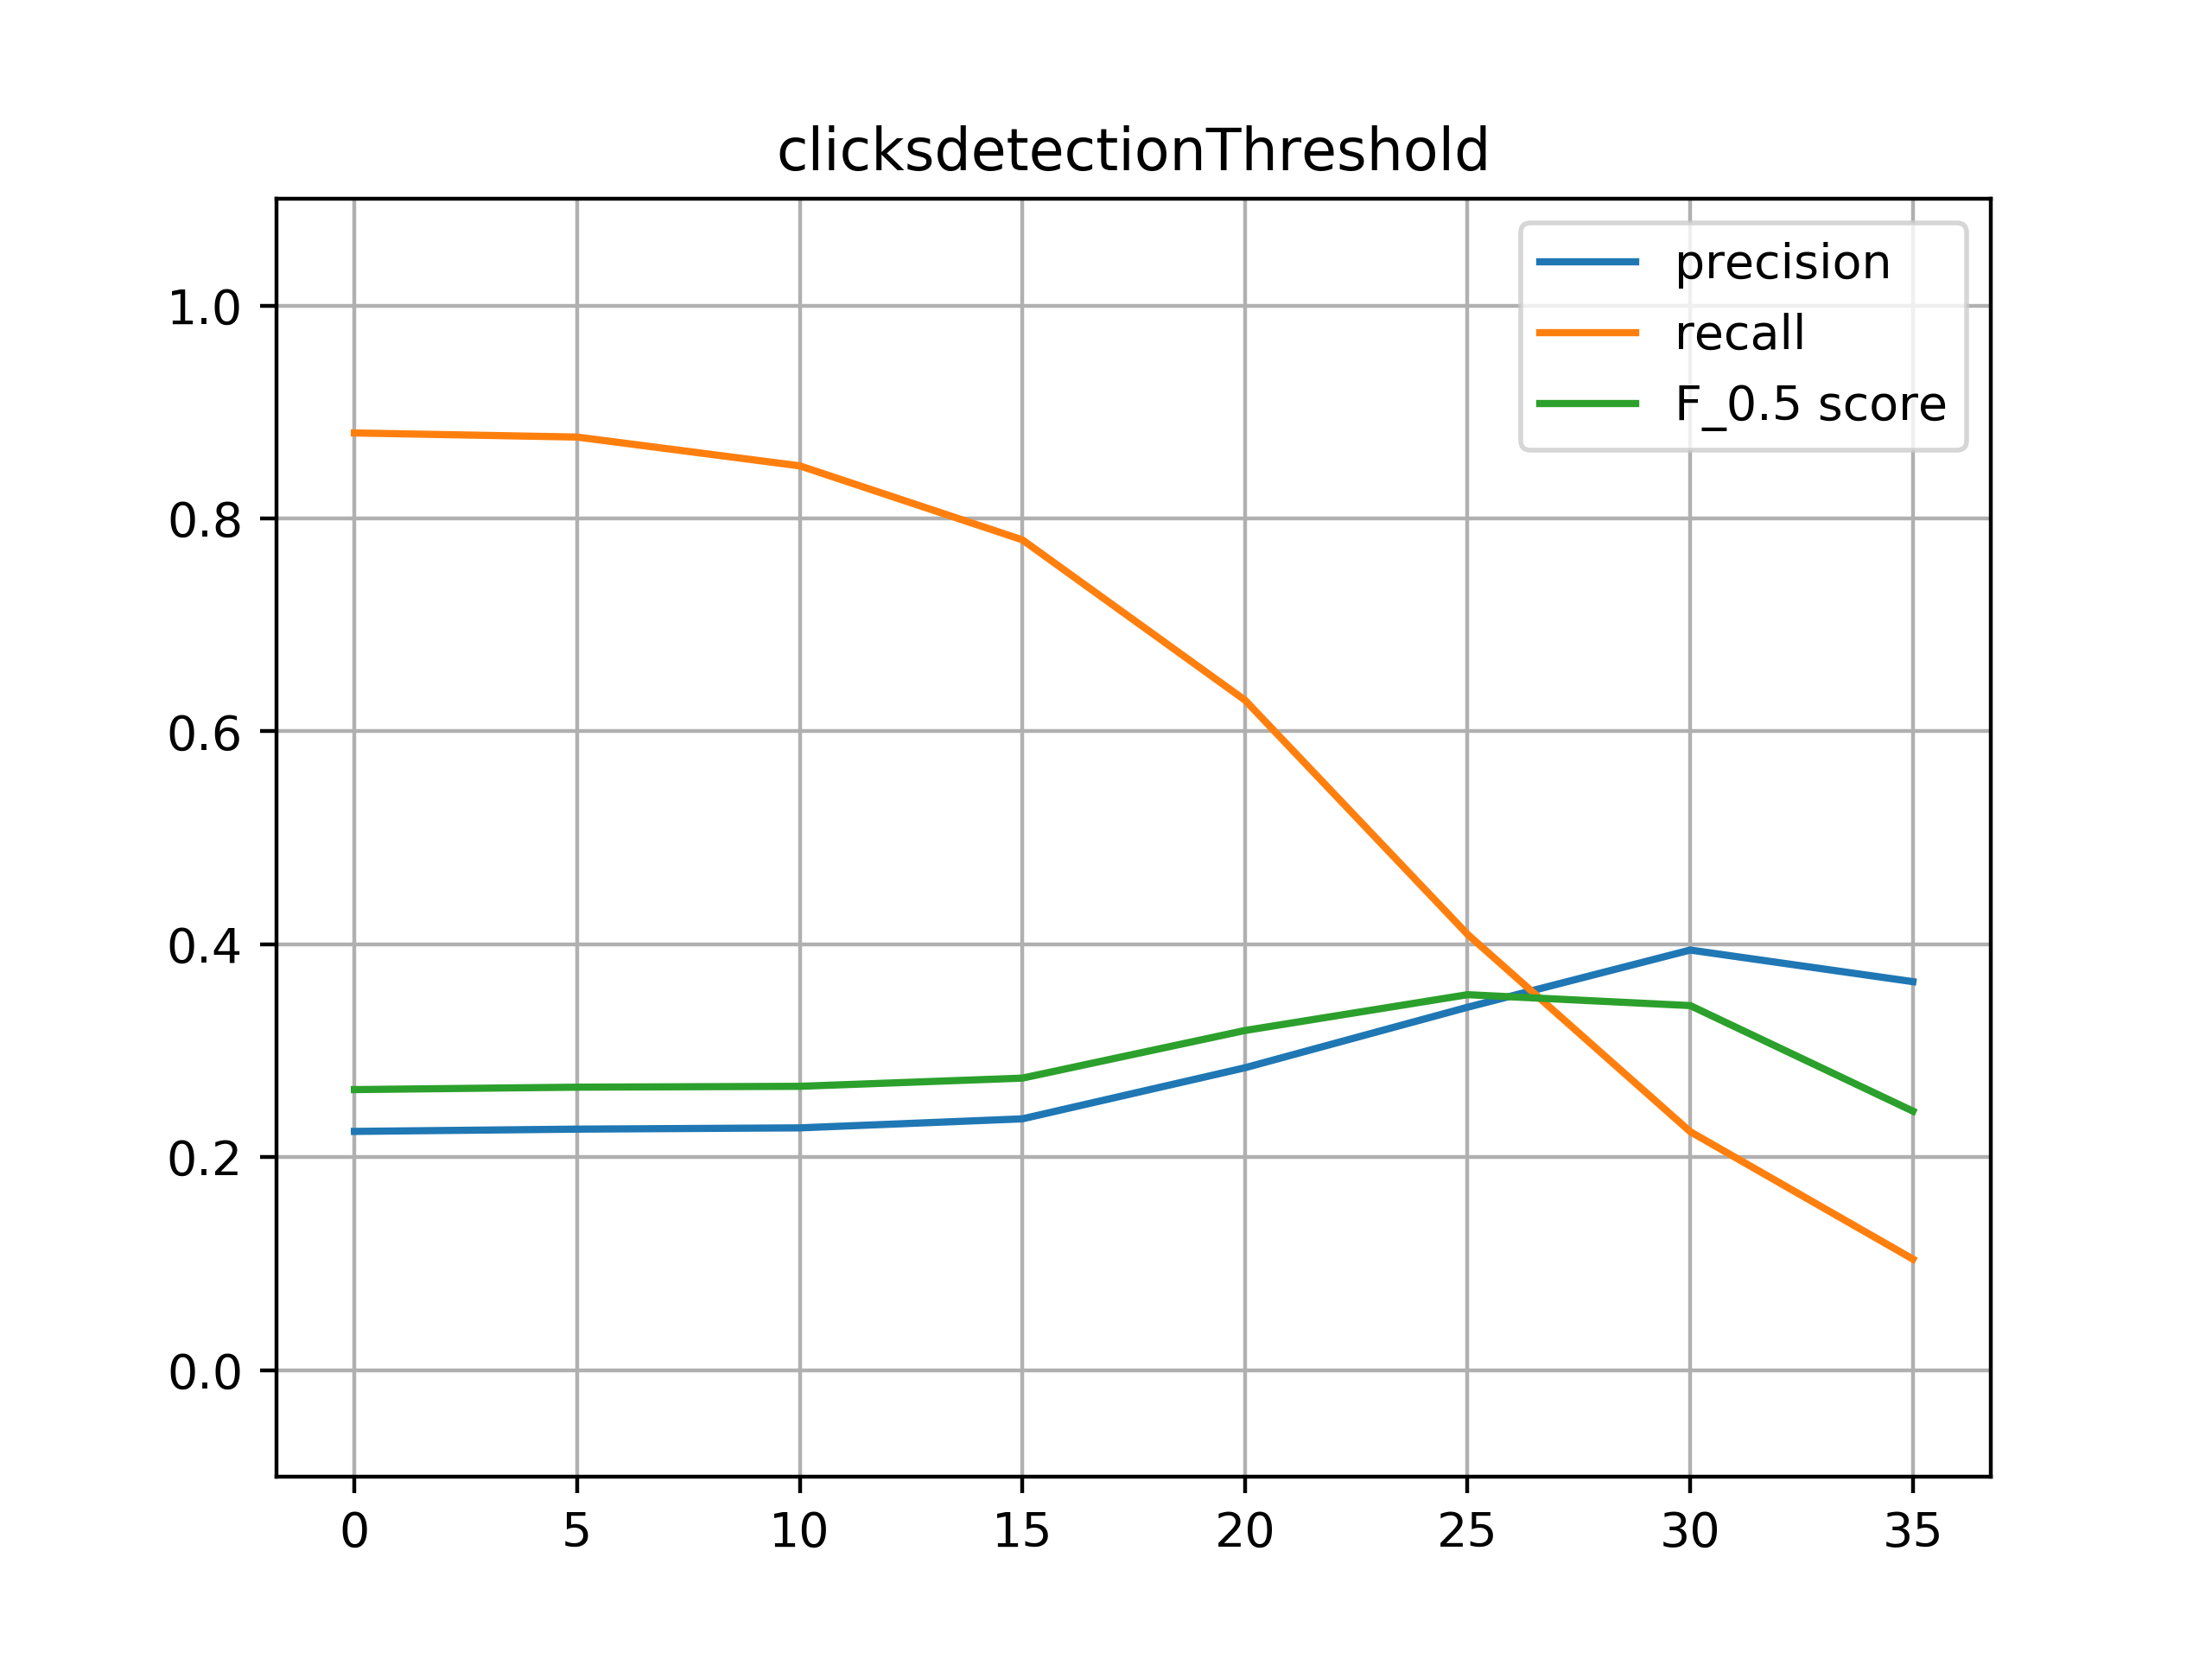
\includegraphics[clip,width=0.7\columnwidth]{Figures/clicksdetectionThreshold.png}% 
	\caption{detectionThreshold parameter sweep results (accuracy, F score and recall)}
	\label{fig:clicksdetectionThreshold}
\end{figure}

The next parameter to be evaluated is order, which is the number of LPC coefficients to use. The parameter was evaluated for the values: [2, 4, 6, 8, 10, 12, 14, 16, 18, 20, 22, 24, 26, 28, 30, 32, 34, 36, 38]. The maximum Fscore value was obtained for a value of 24 and the result was a value of over 0.4.

\begin{figure}[H]
	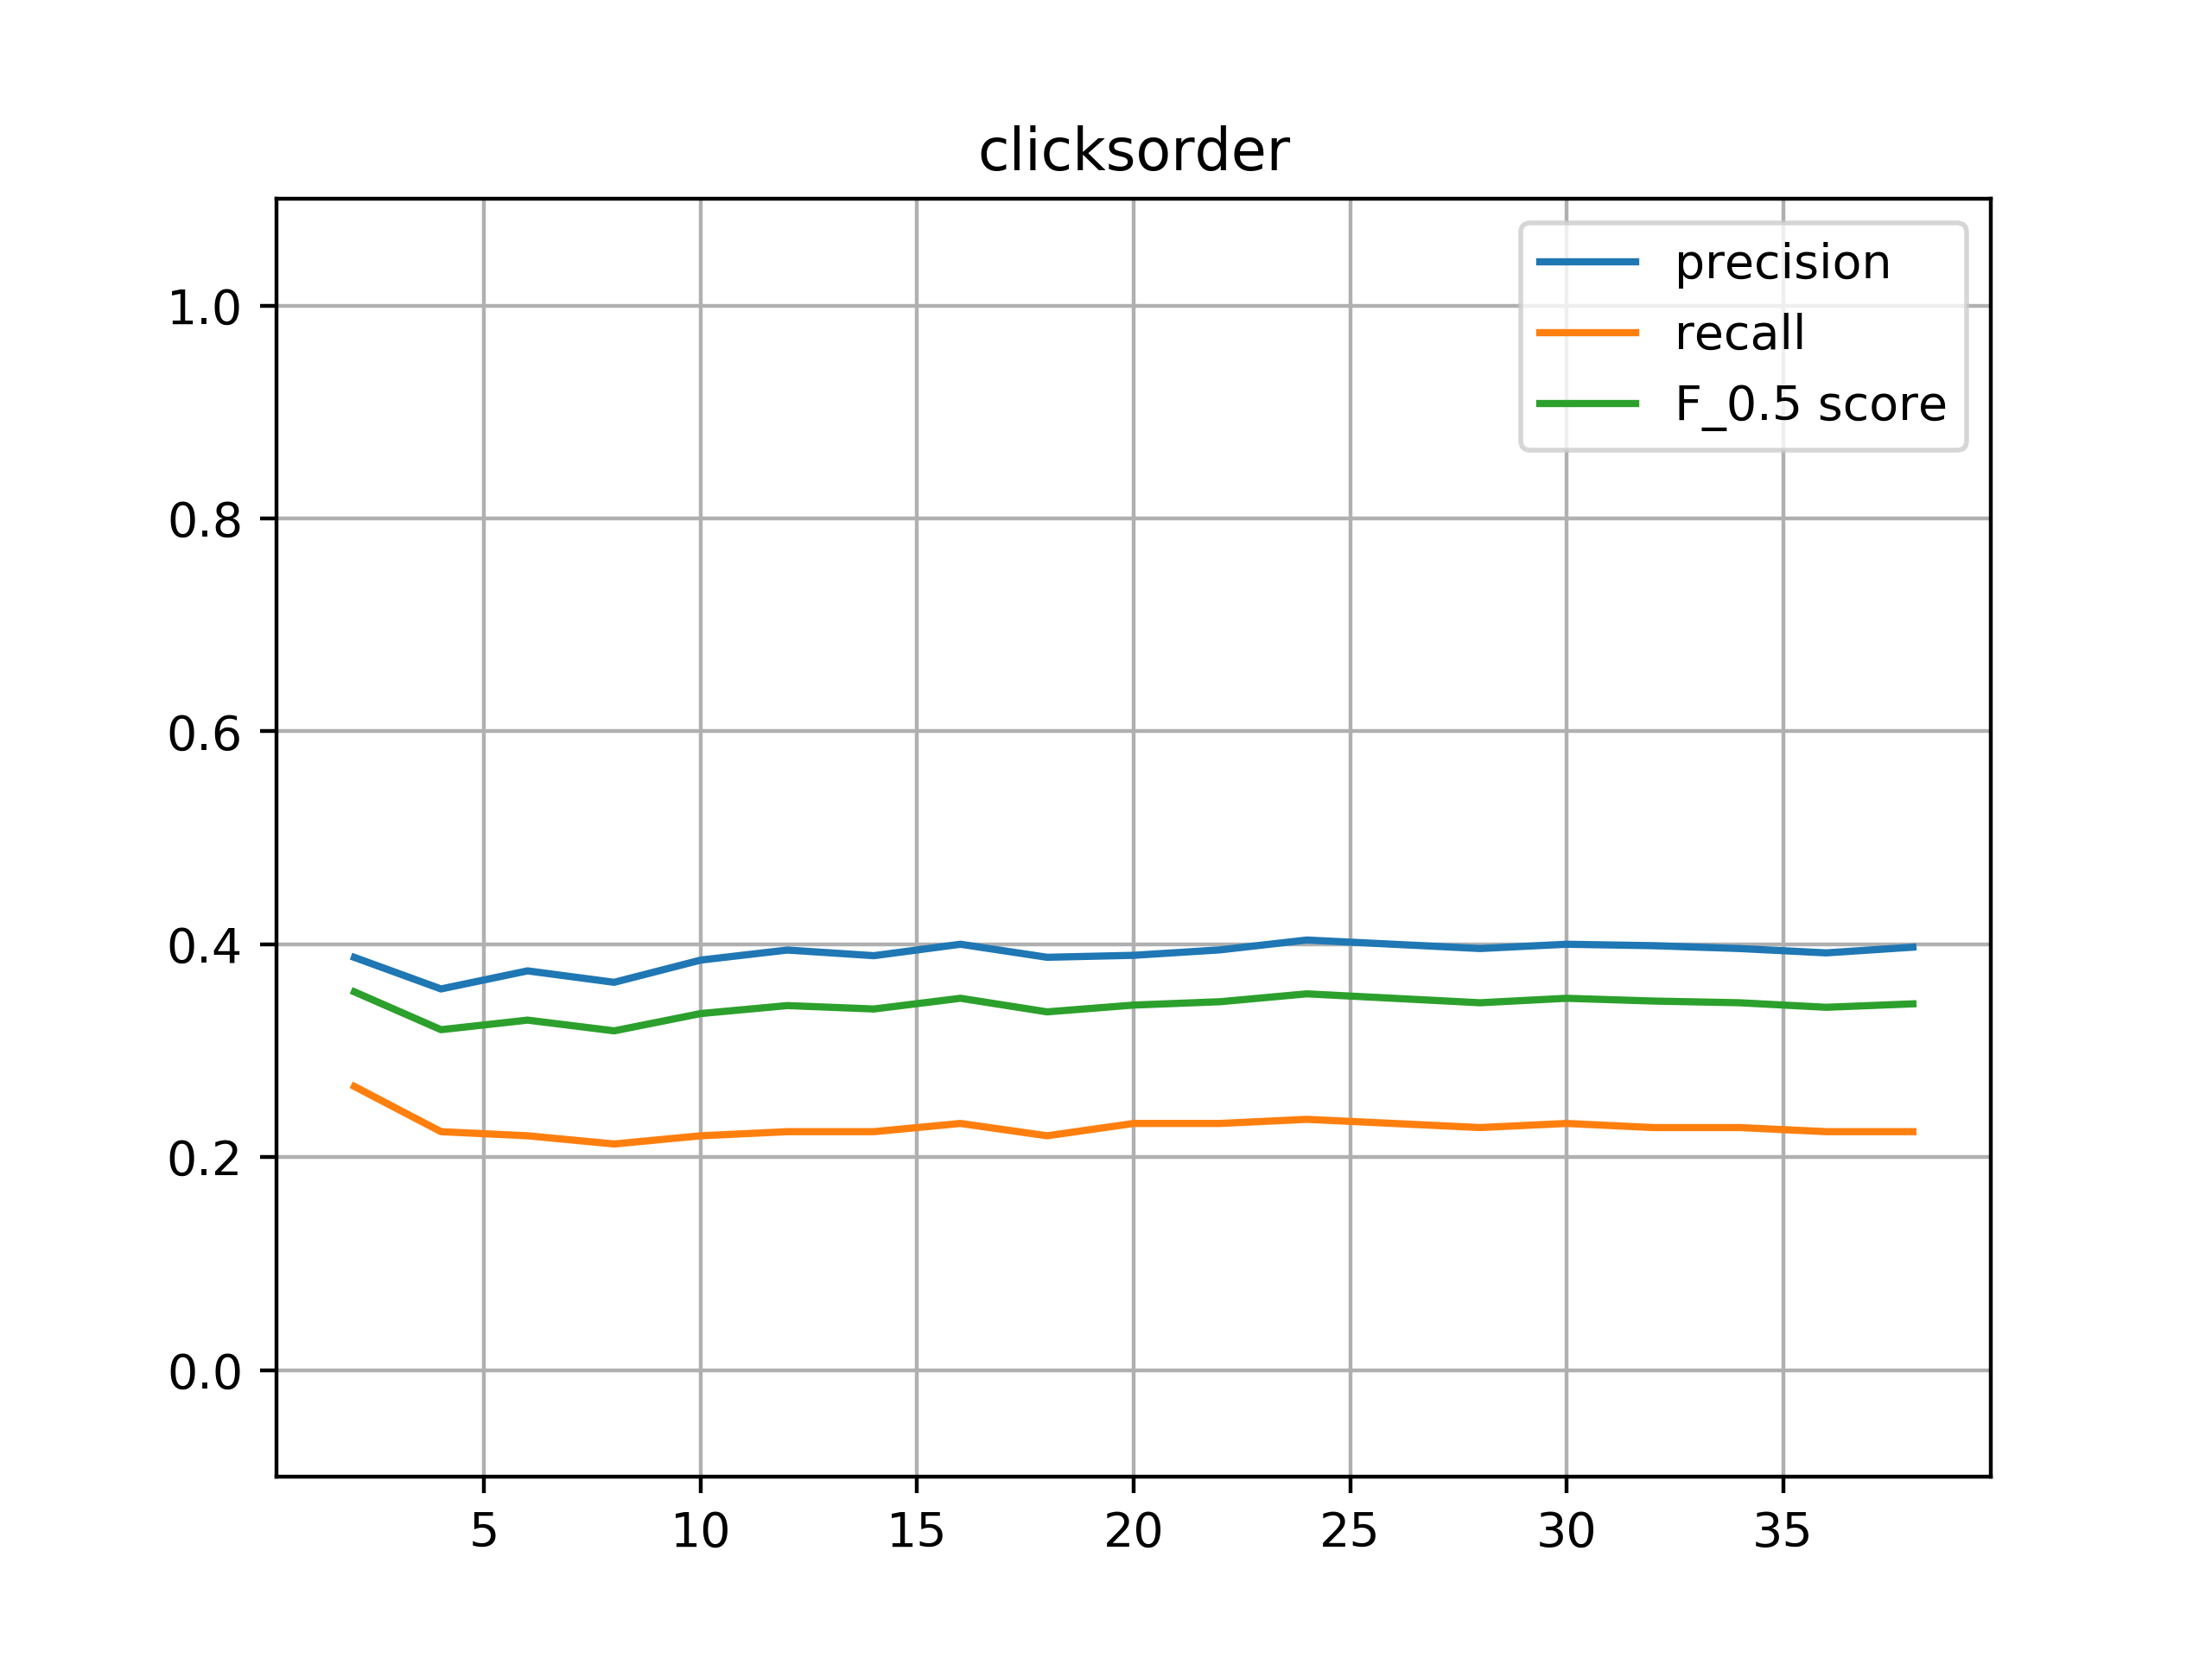
\includegraphics[clip,width=0.7\columnwidth]{Figures/clicksorder.png}% 
	\caption{order parameter sweep results (accuracy, F score and recall)}
	\label{fig:clicksorder}
\end{figure}

The next parameter to be evaluated is powerEstimationThreshold. In the algorithm, the noisy excitation is clipped to powerEstimationThreshold times its median. The parameter was evaluated for the values: [2, 4, 6, 8, 10, 12, 14]. The maximum Fscore value was obtained for a value of 10 and the result was a value of over 0.35.

\begin{figure}[H]
	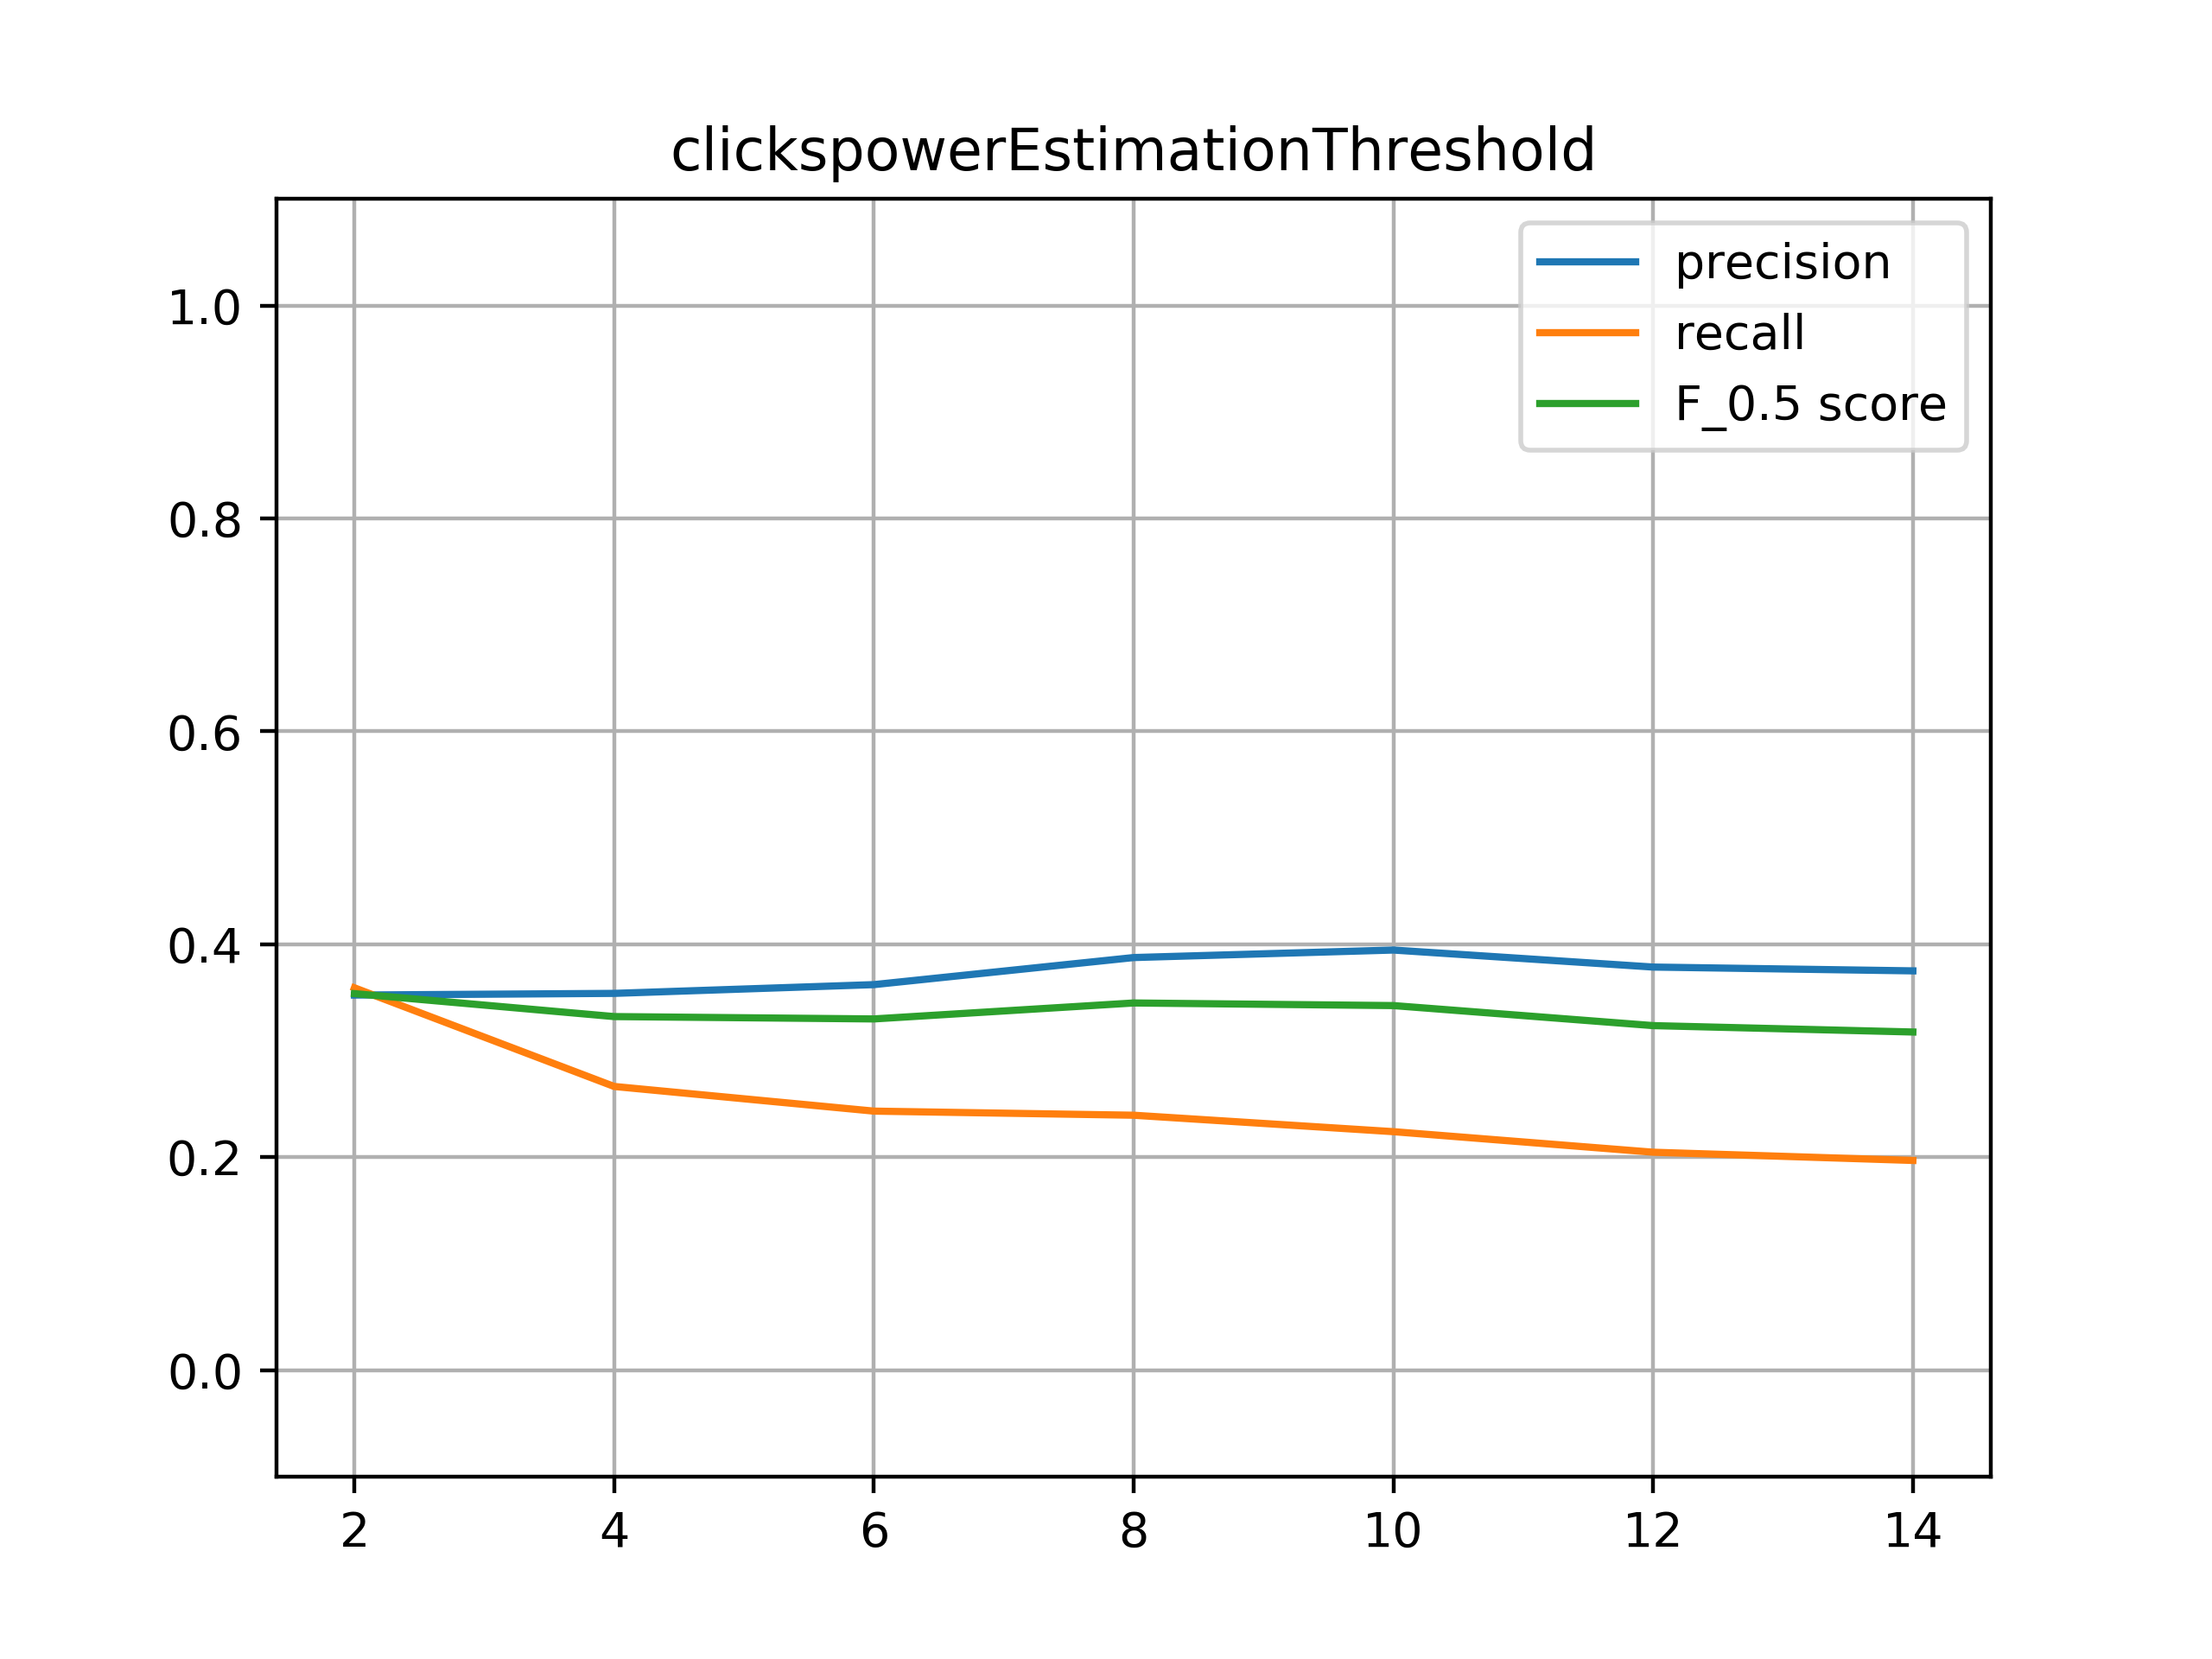
\includegraphics[clip,width=0.7\columnwidth]{Figures/clickspowerEstimationThreshold.png}% 
	\caption{powerEstimationThreshold parameter sweep results (accuracy, F score and recall)}
	\label{fig:clickspowerEstimationThreshold}
\end{figure}

The next parameter to be evaluated is silenceThreshold. The value represents the threshold to skip silent frames. The parameter was evaluated for the values: [-70, -60, -50, -40, -30, -20, -10]. The maximum Fscore value was obtained for a value of -60 and the result was a value of over 0.35.

\begin{figure}[H]
	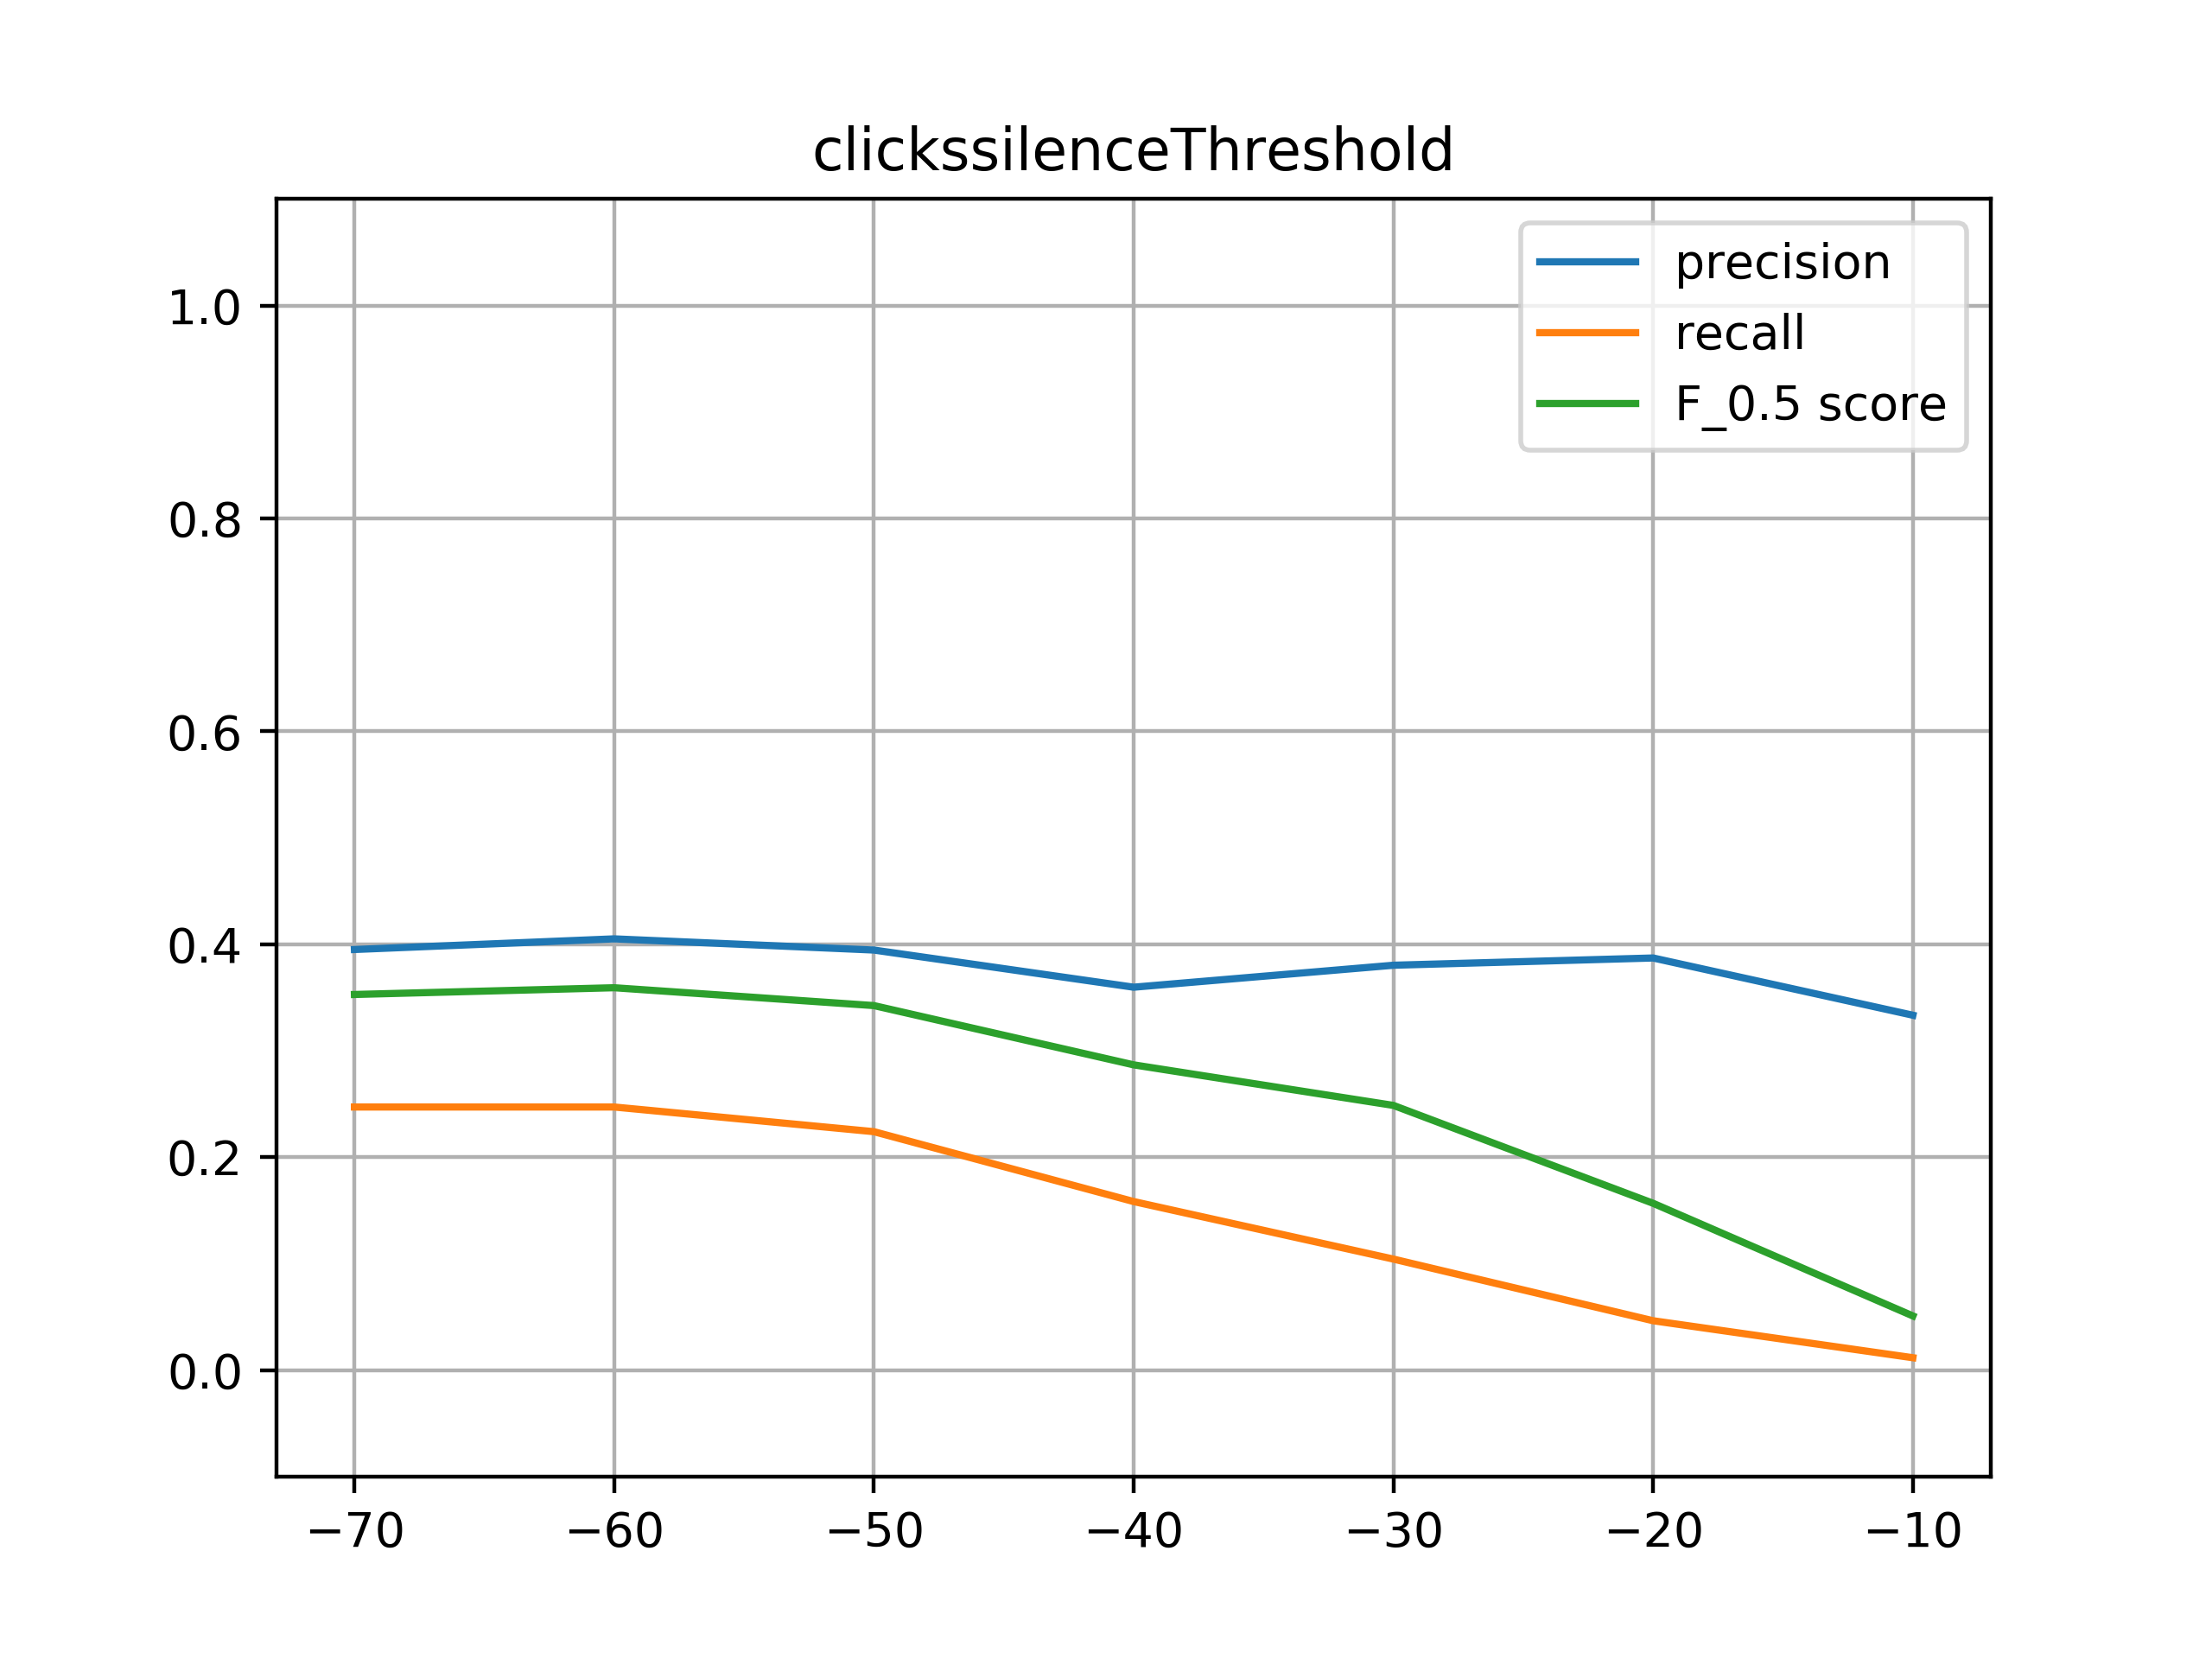
\includegraphics[clip,width=0.7\columnwidth]{Figures/clickssilenceThreshold.png}% 
	\caption{silenceThreshold parameter sweep results (accuracy, F score and recall)}
	\label{fig:clickssilenceThreshold}
\end{figure}

\section{Noise bursts detection evaluation}
For the noise bursts detection algorithm two values were sweeped: alpha value and threshold. The alpha value is the alpha value for Exponential Moving Average threshold estimation. The valuye was sweeped for the range: [0.1, 0.2, 0.3, 0.4, 0.5, 0.6, 0.7, 0.8, 0.9] and the best value of Fscore was achieved for 0.1.

\begin{figure}[H]
	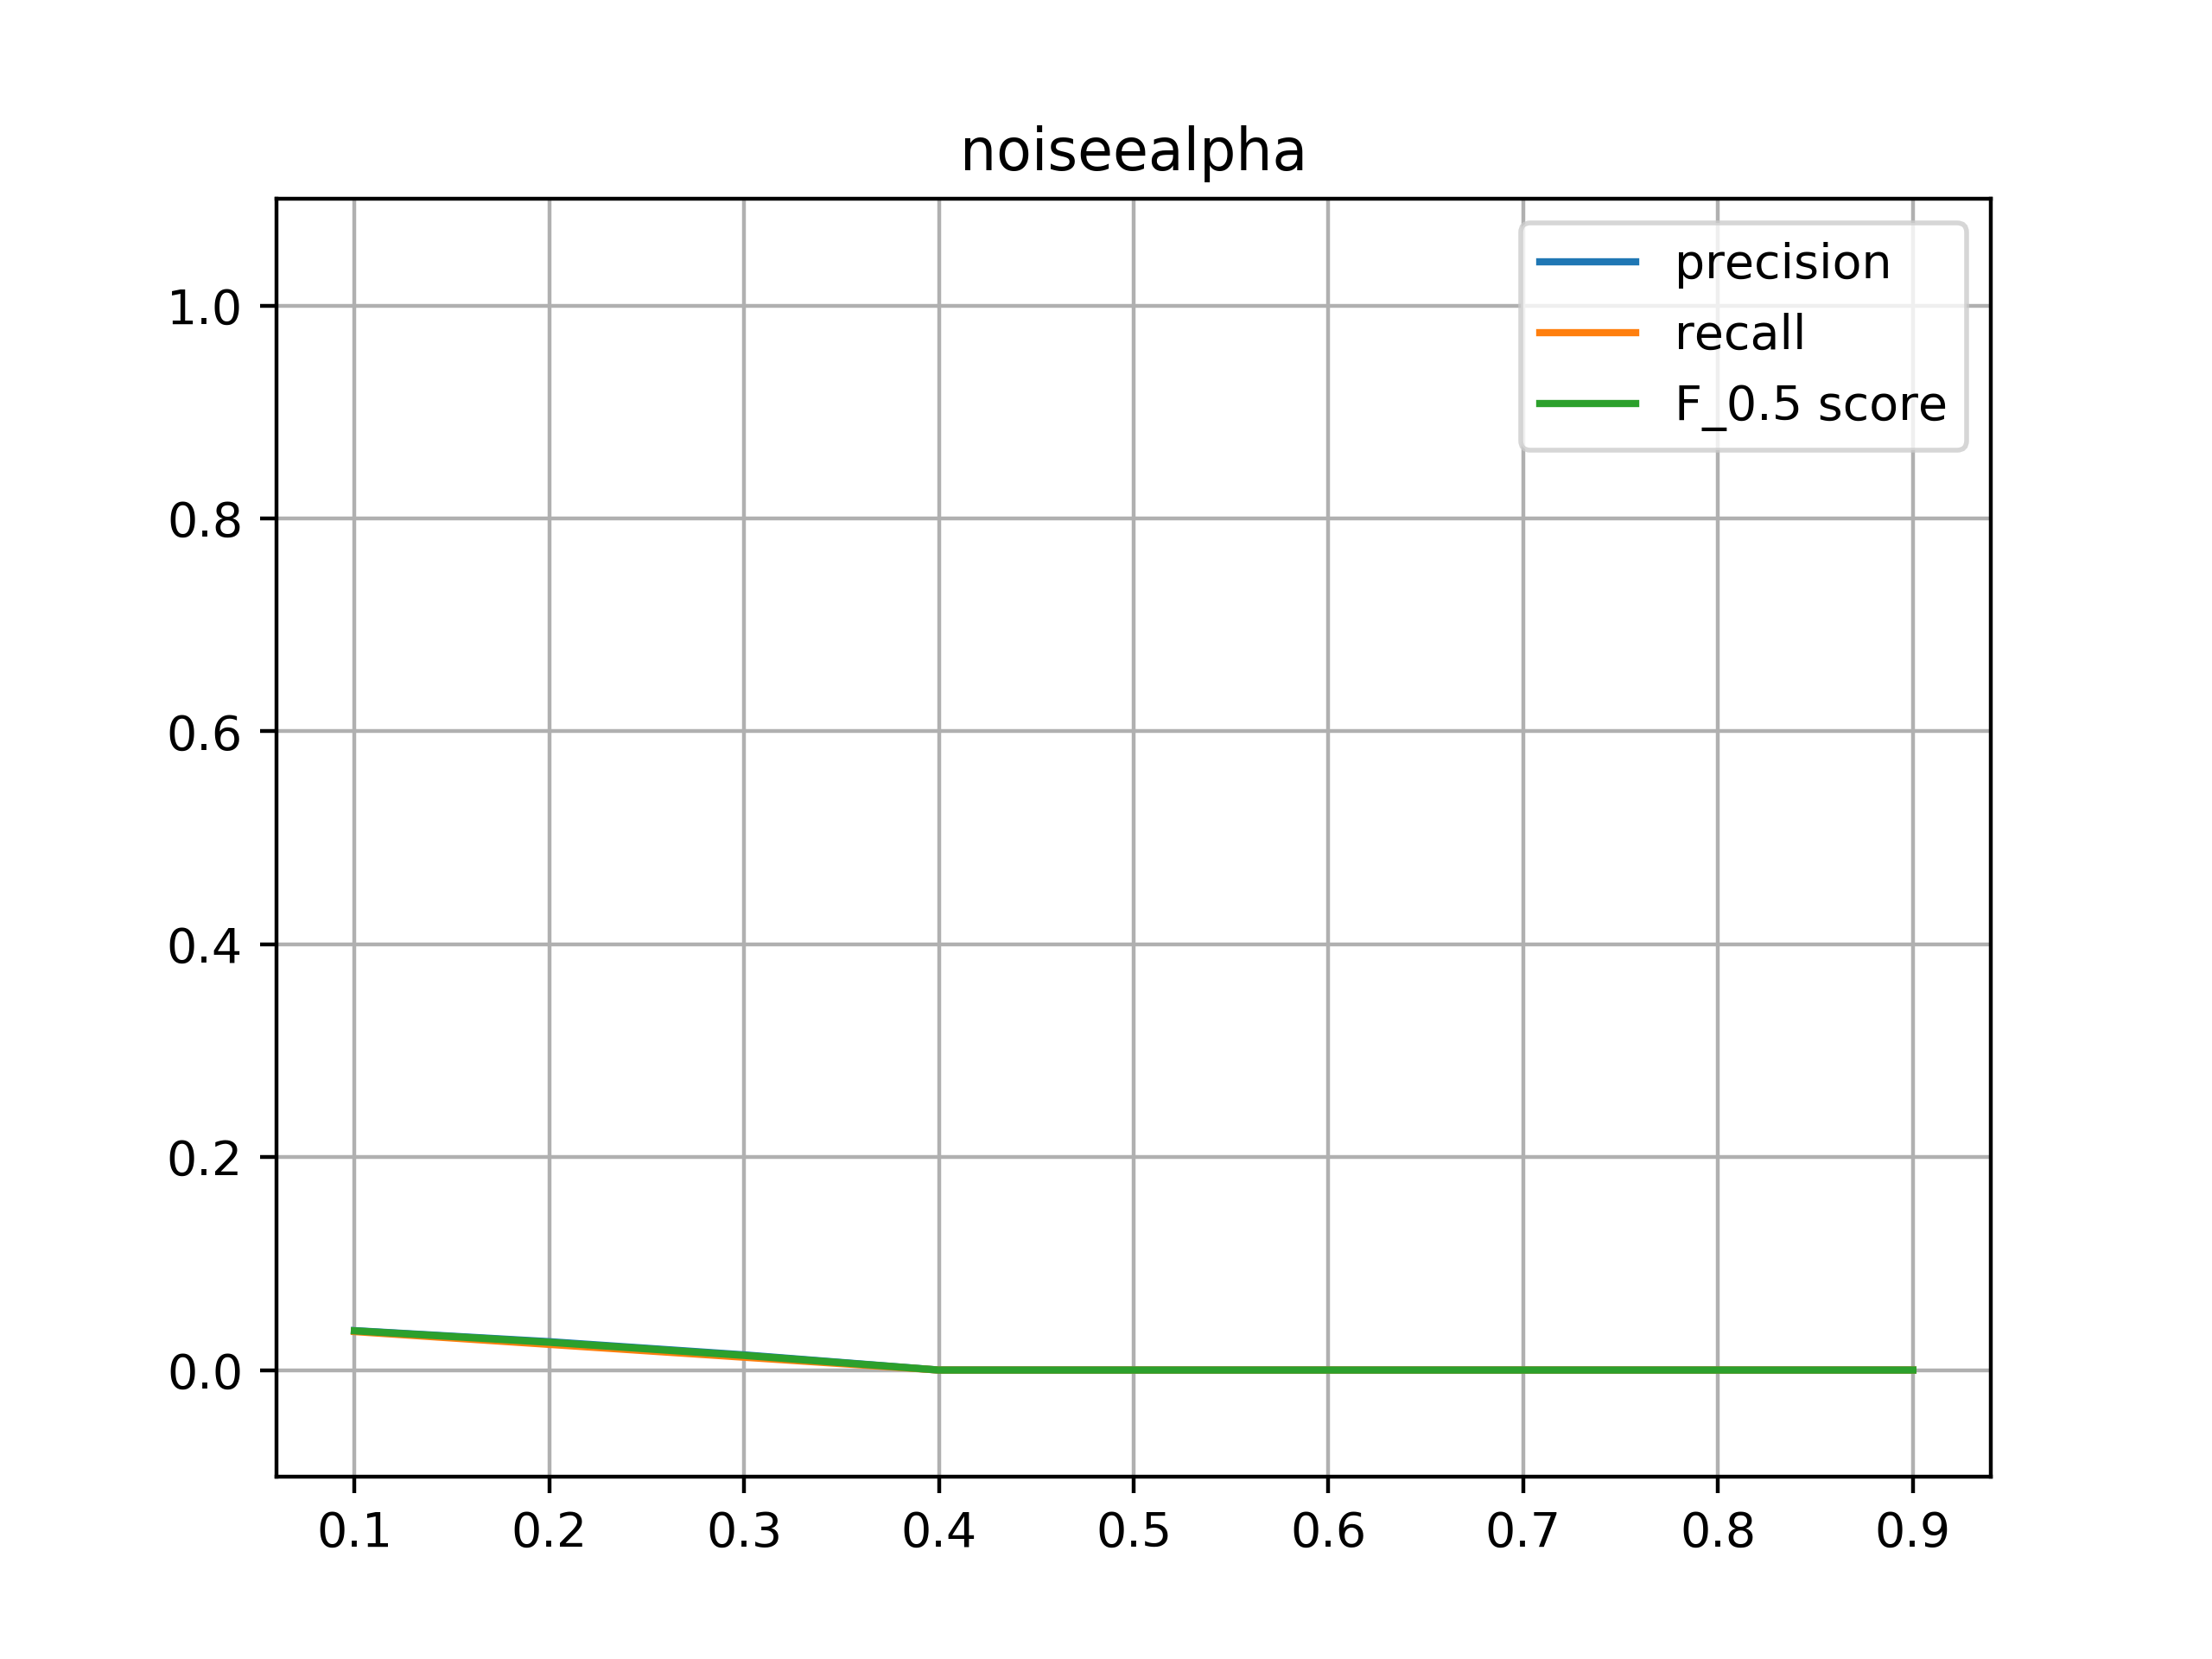
\includegraphics[clip,width=0.7\columnwidth]{Figures/noiseealpha.png}% 
	\caption{alpha parameter sweep results (accuracy, F score and recall)}
	\label{fig:noiseealpha}
\end{figure}

The threshold value represent the threshold to skip silent frames. The parameter was swept for the following values: [-10, -8, -6, -4, -2, 0, 2, 4, 6, 8, 10] and the best results were obtained for the value of 4 giving an accuracy of 0.3.

\begin{figure}[H]
	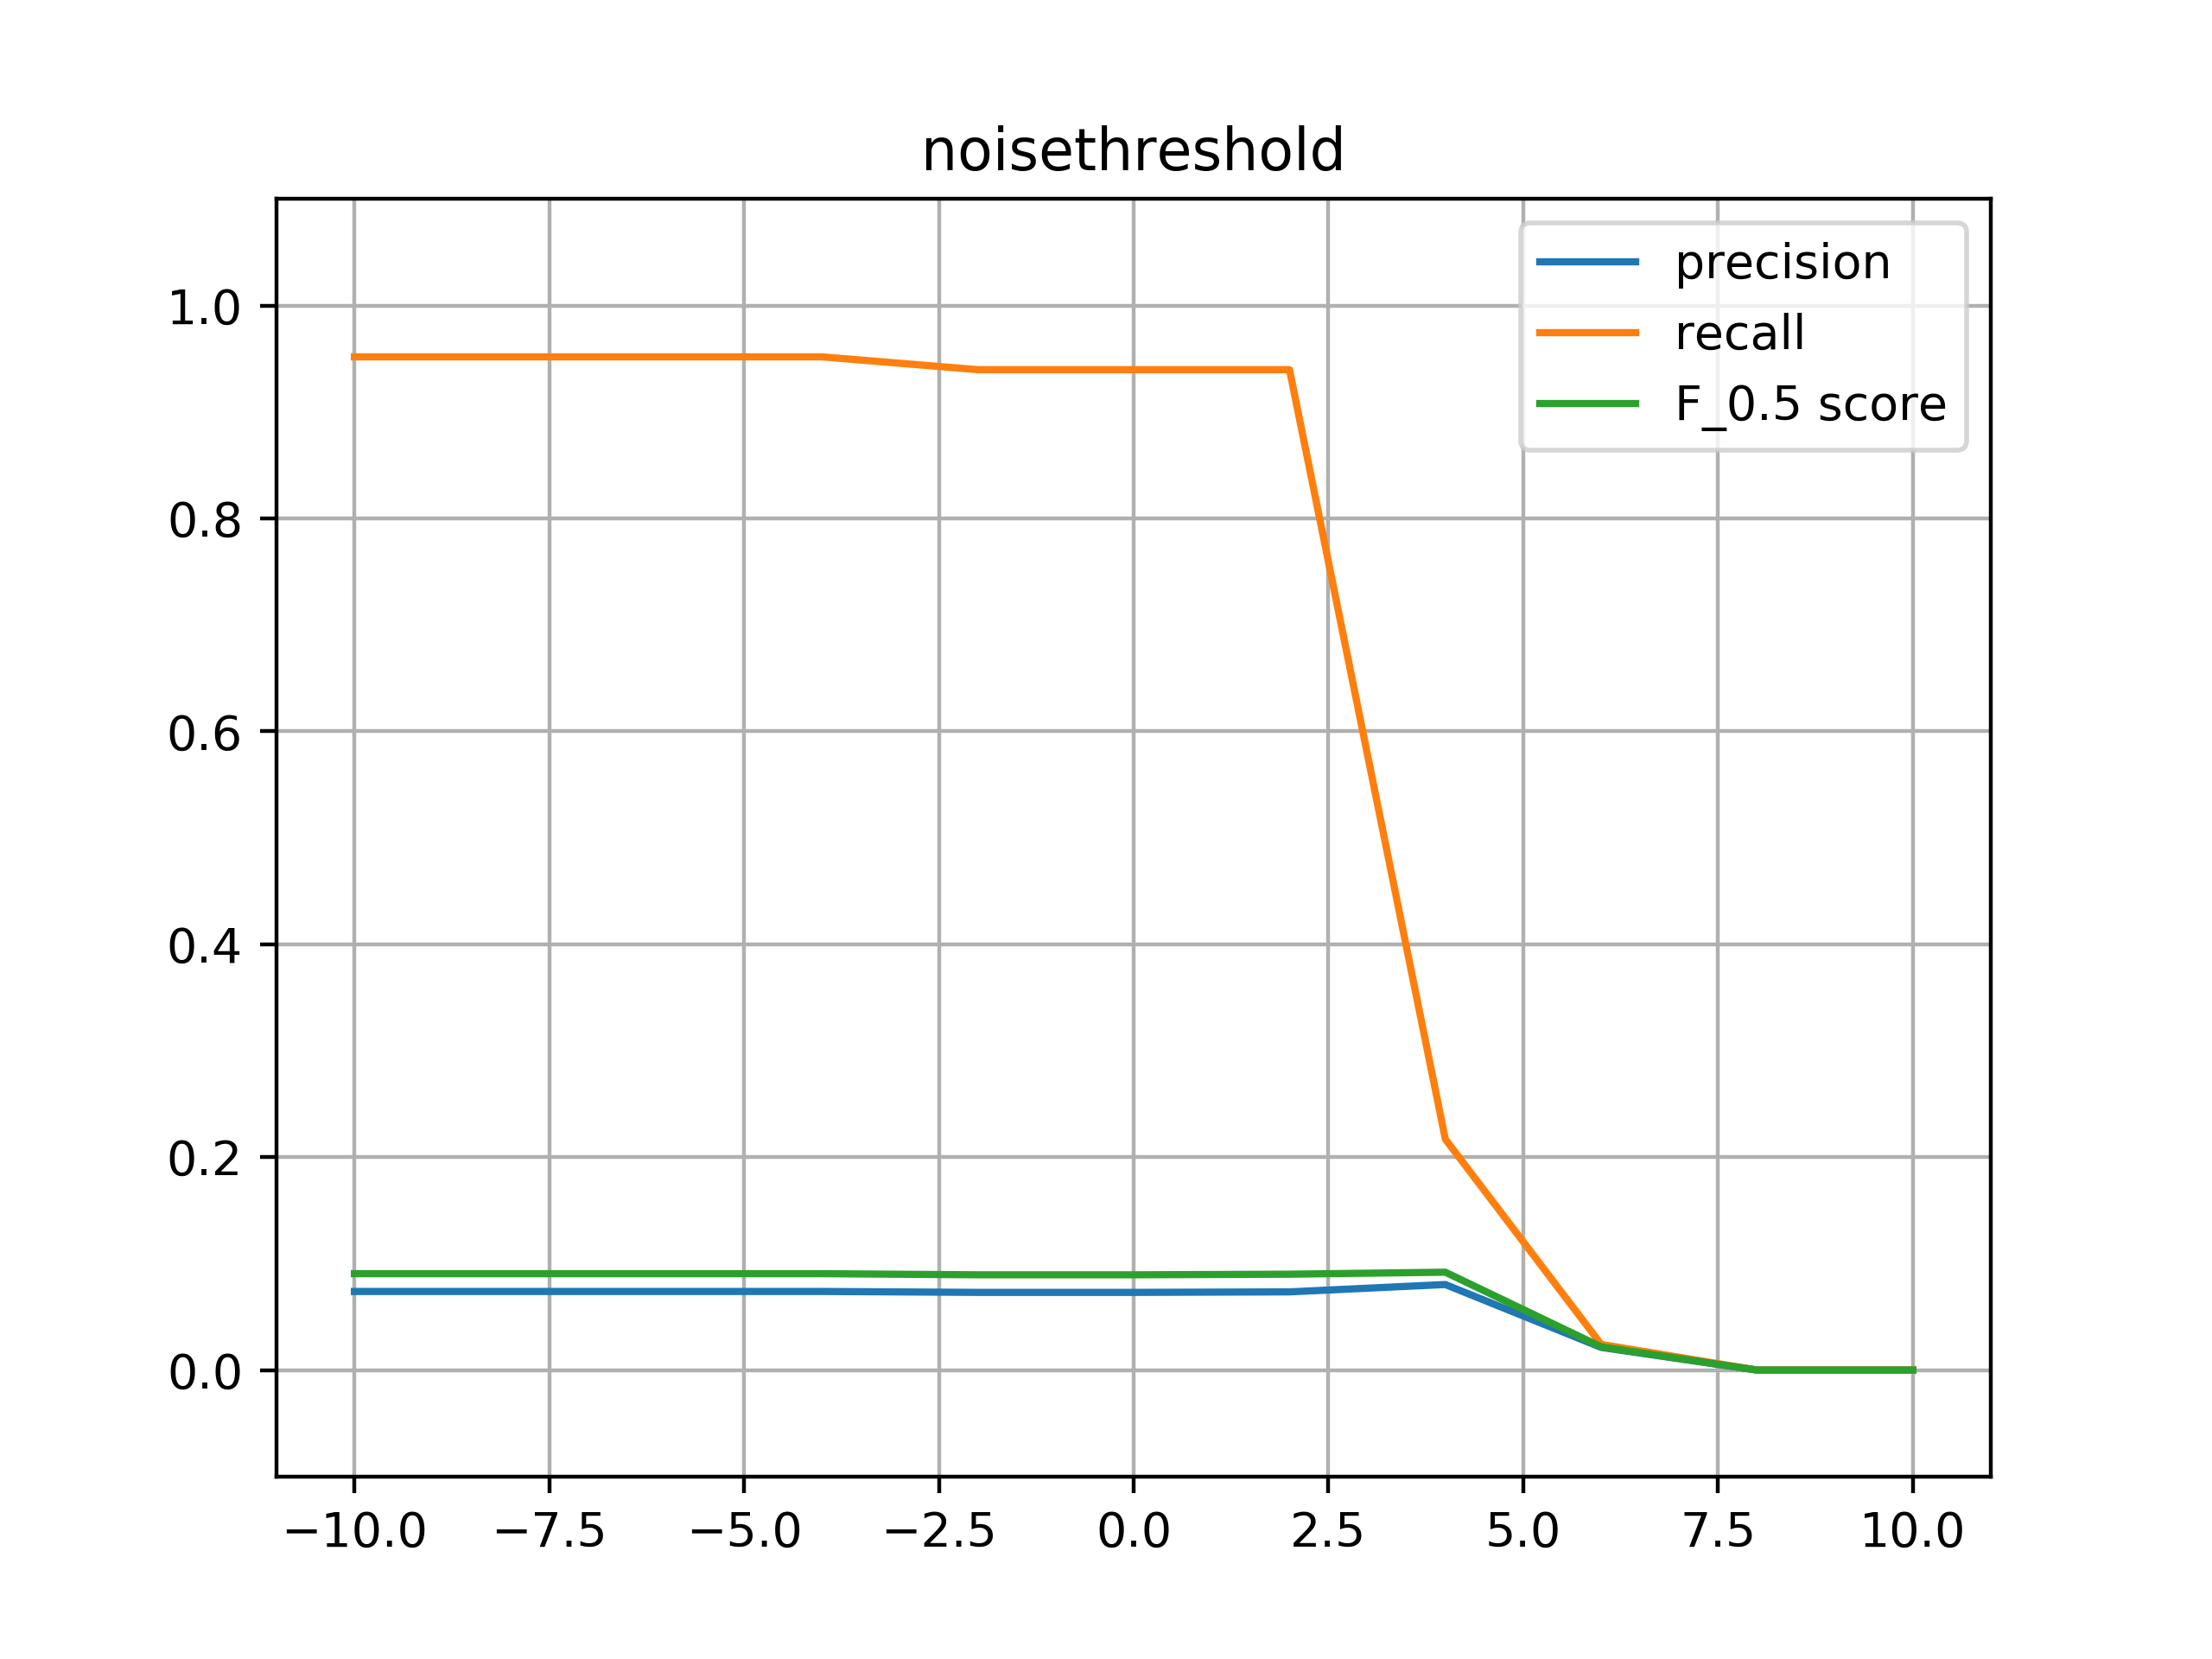
\includegraphics[clip,width=0.7\columnwidth]{Figures/noisethreshold.png}% 
	\caption{threshold parameter sweep results (accuracy, F score and recall)}
	\label{fig:noisethreshold}
\end{figure}

\section{Saturation detection evaluation}
For the saturation evaluation, the parameters differentialThreshold, energyThreshold and minimumDuration. The first parameter represents minimum difference between contiguous samples of the salturated regions. The parameter was swept for the values: [0.001, 0.005, 0.01, 0.05, 0.1, 0.5, 1, 5, 10]. And the best results in Fscore were obtained for high values such as 5 or 10, but, if precision was to be priotitized, the smallest value wouyld give the best results. 

\begin{figure}[H]
	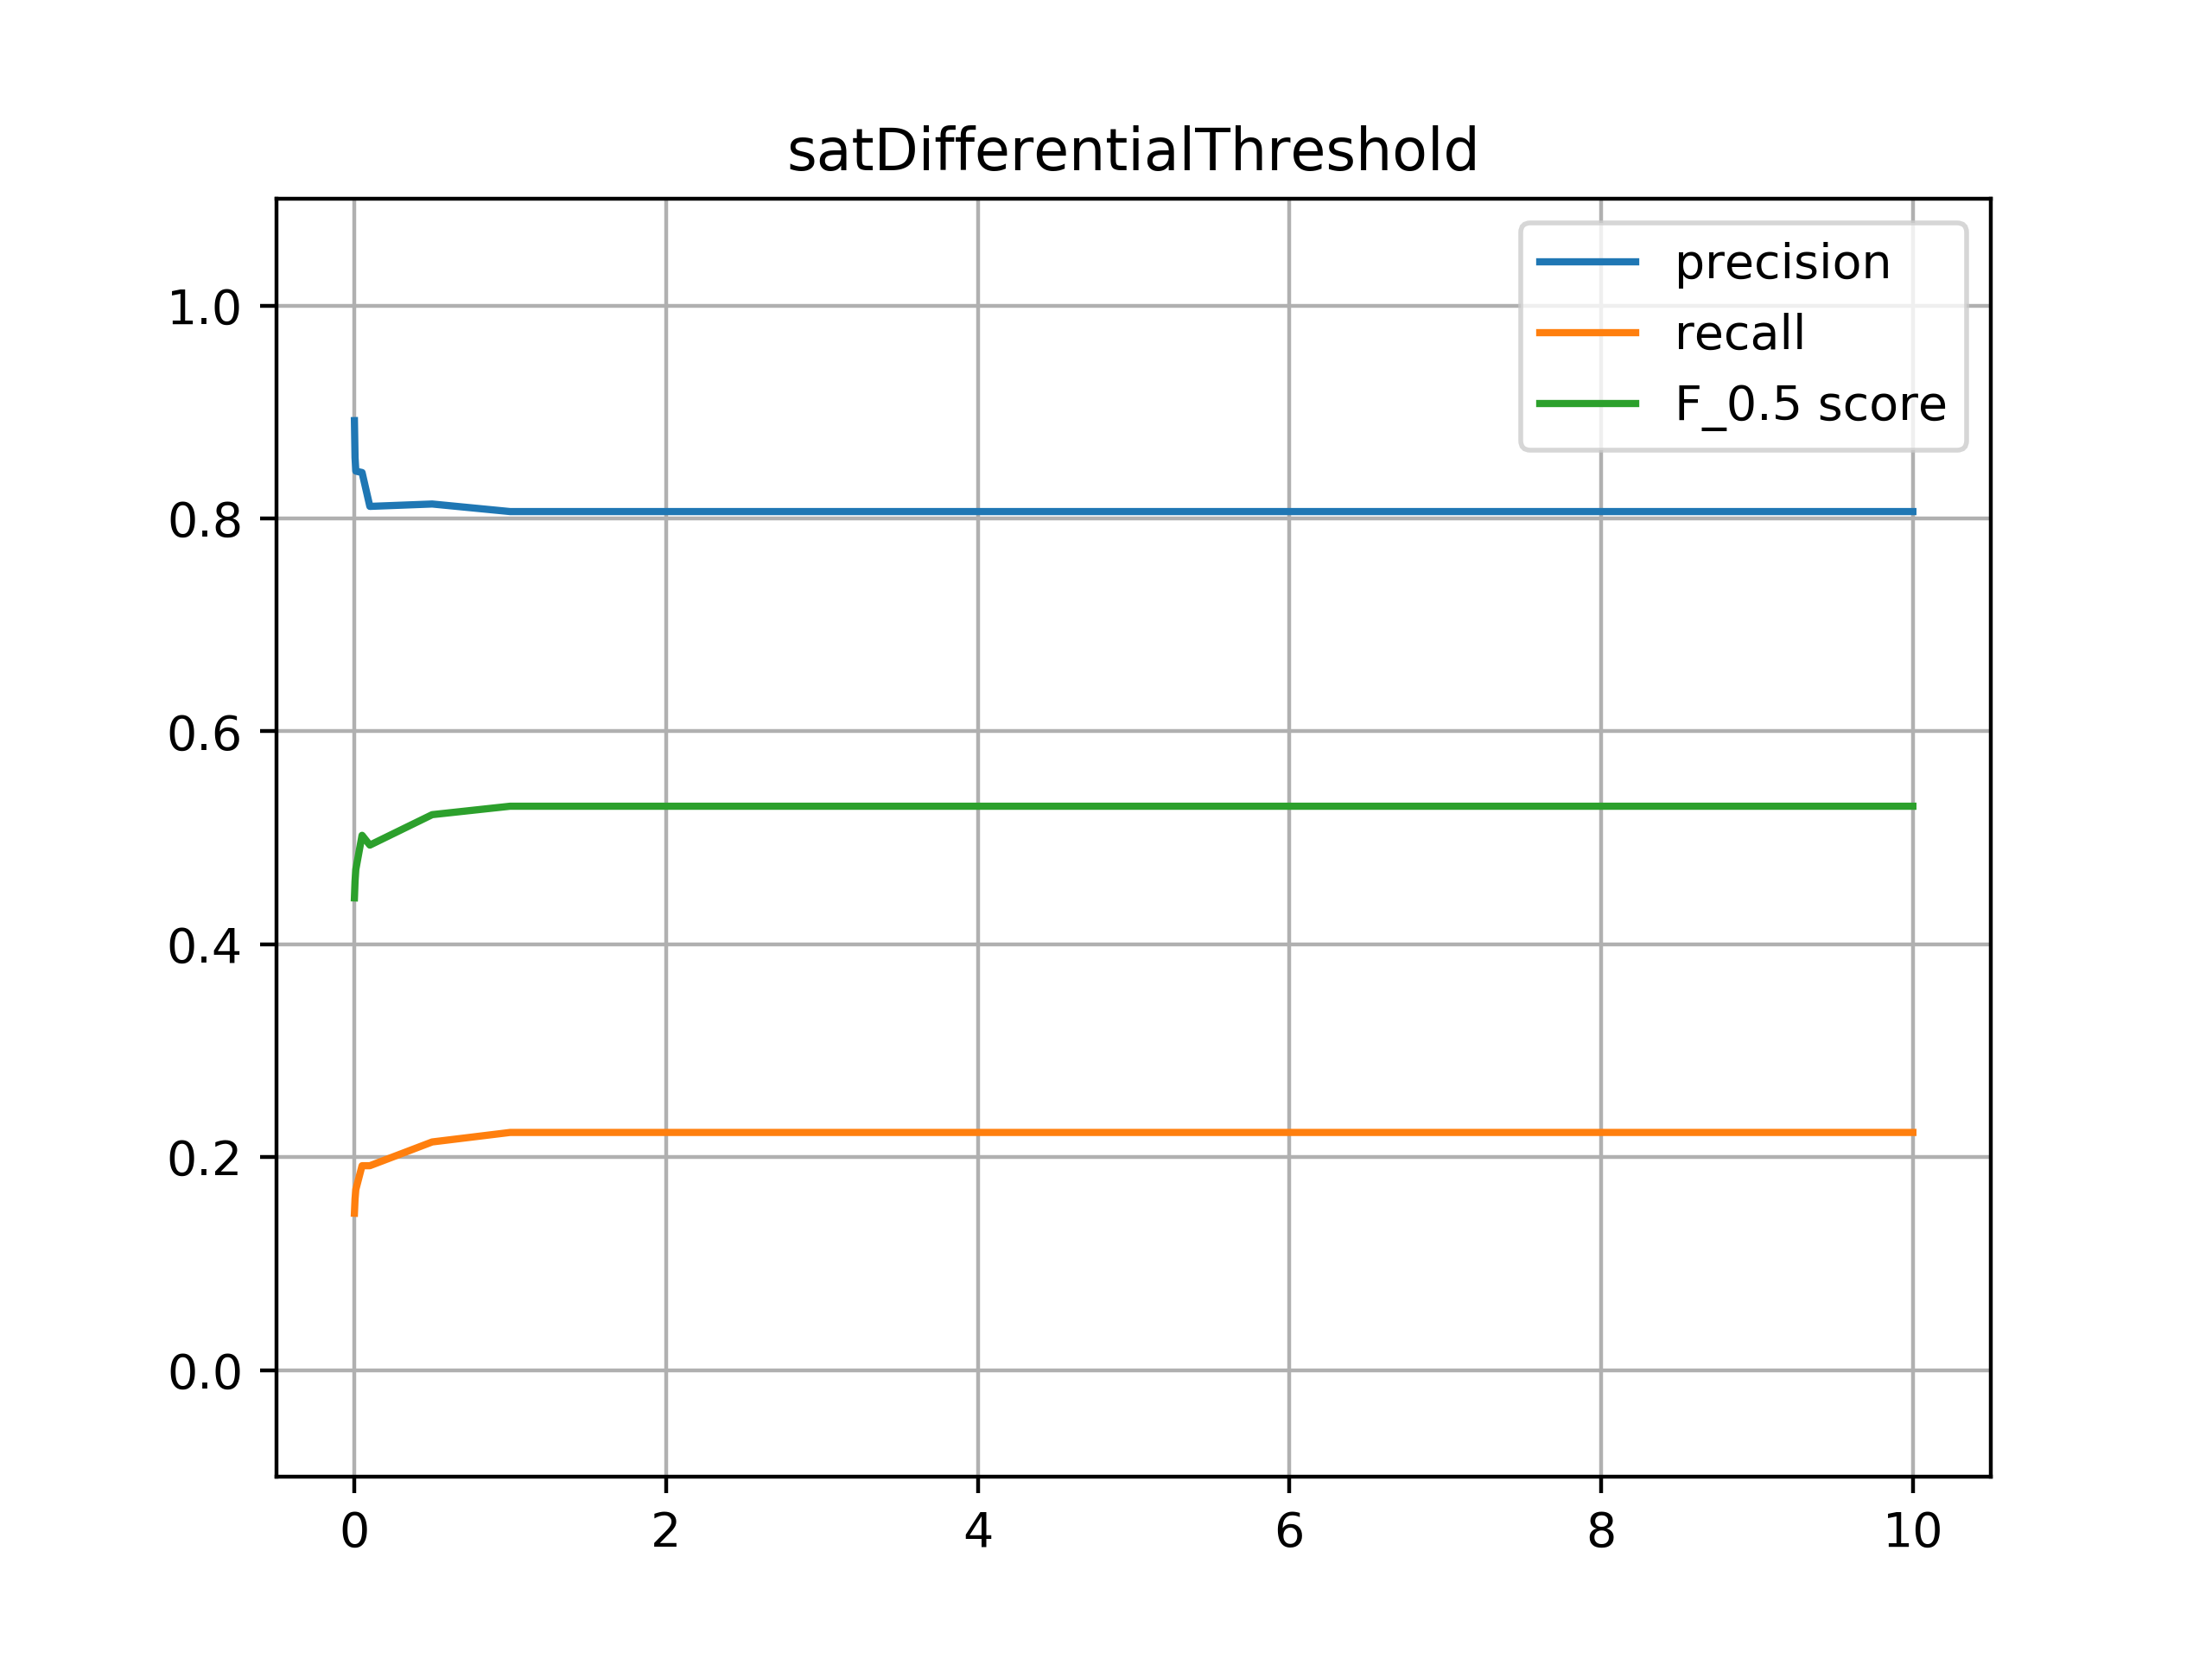
\includegraphics[clip,width=0.7\columnwidth]{Figures/satDifferentialThreshold.png}% 
	\caption{differentialThreshold parameter sweep results (accuracy, F score and recall)}
	\label{fig:satDifferentialThreshold}
\end{figure}

The second parameter is energyThreshold which is the minimum energy for the algorithm to assume a region as saturated. The value was swept for the values: [-30, -20, -10, -7, -5, -3, -1, -0.01] and the best Fscore results were obtainesd for -5 dB.

\begin{figure}[H]
	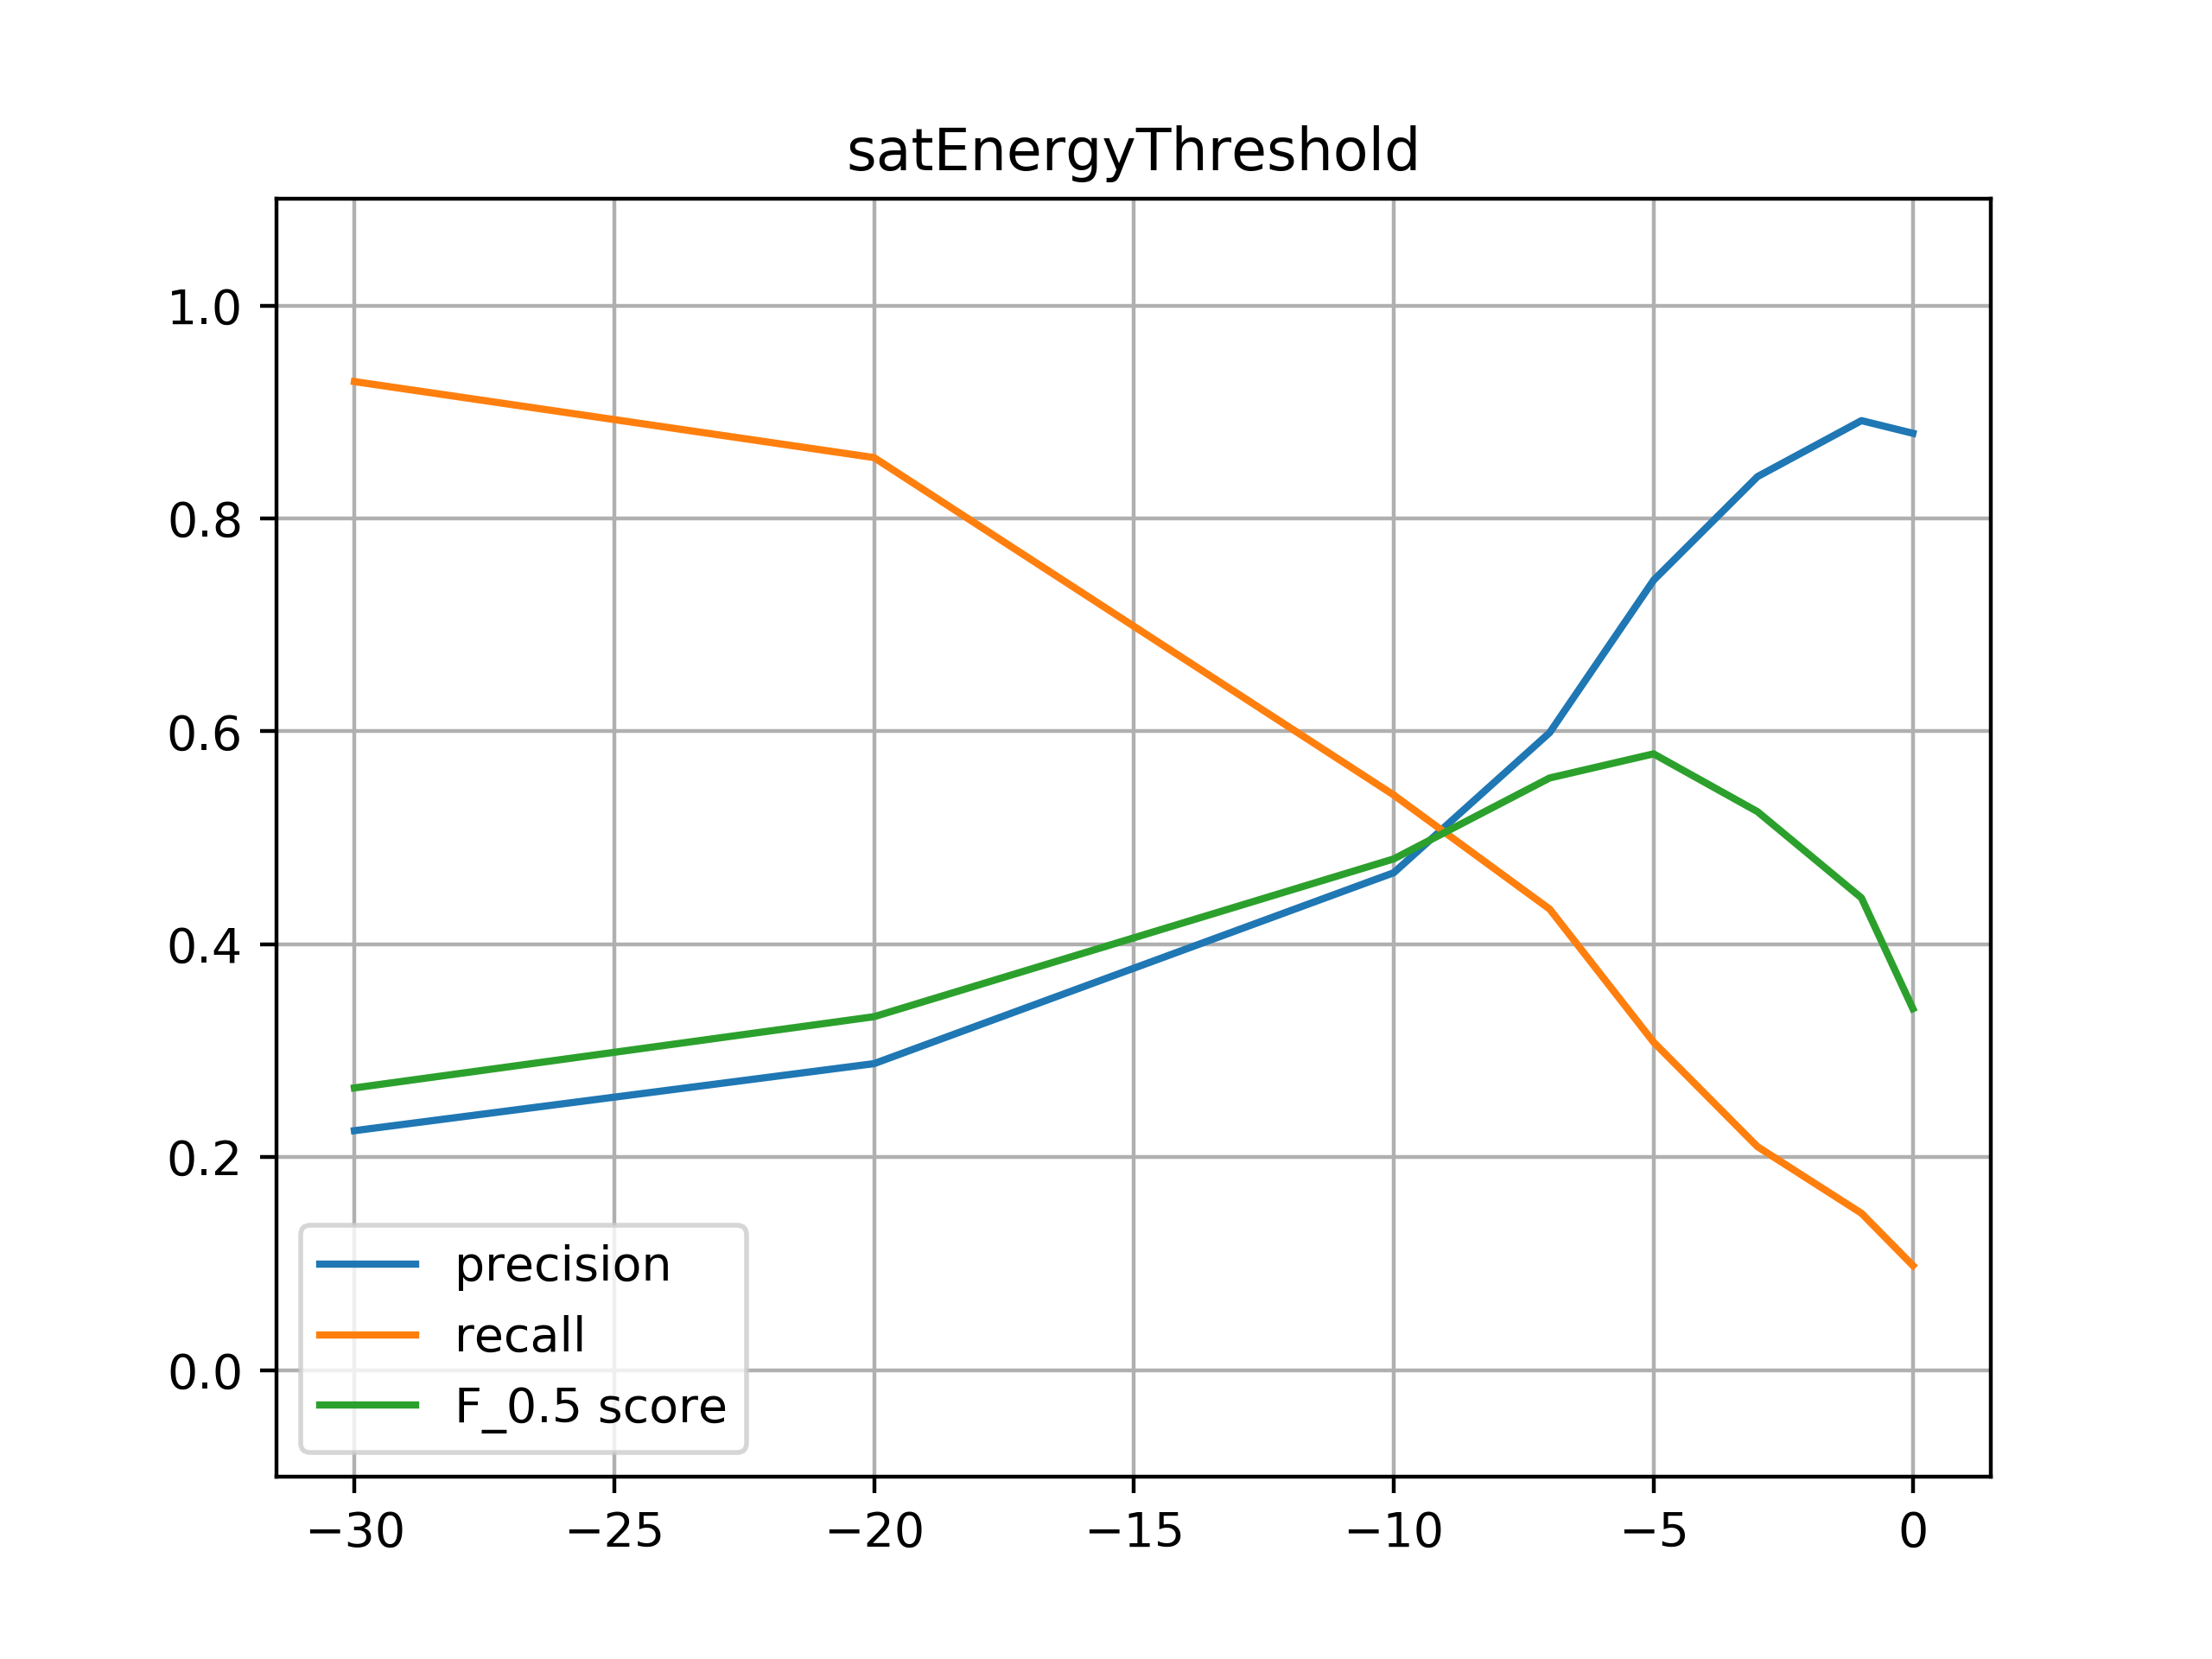
\includegraphics[clip,width=0.7\columnwidth]{Figures/satEnergyThreshold.png}% 
	\caption{energyThreshold parameter sweep results (accuracy, F score and recall)}
	\label{fig:satEnergyThreshold}
\end{figure}

The last parameter is minimumDuration, which is the time threshold for the algorithm to detect a saturated region. The parameter was swept for the values: [0.001, 0.005, 0.01, 0.05, 0.1, 0.5, 1] and the best results were obtained for 0.001.

\begin{figure}[H]
	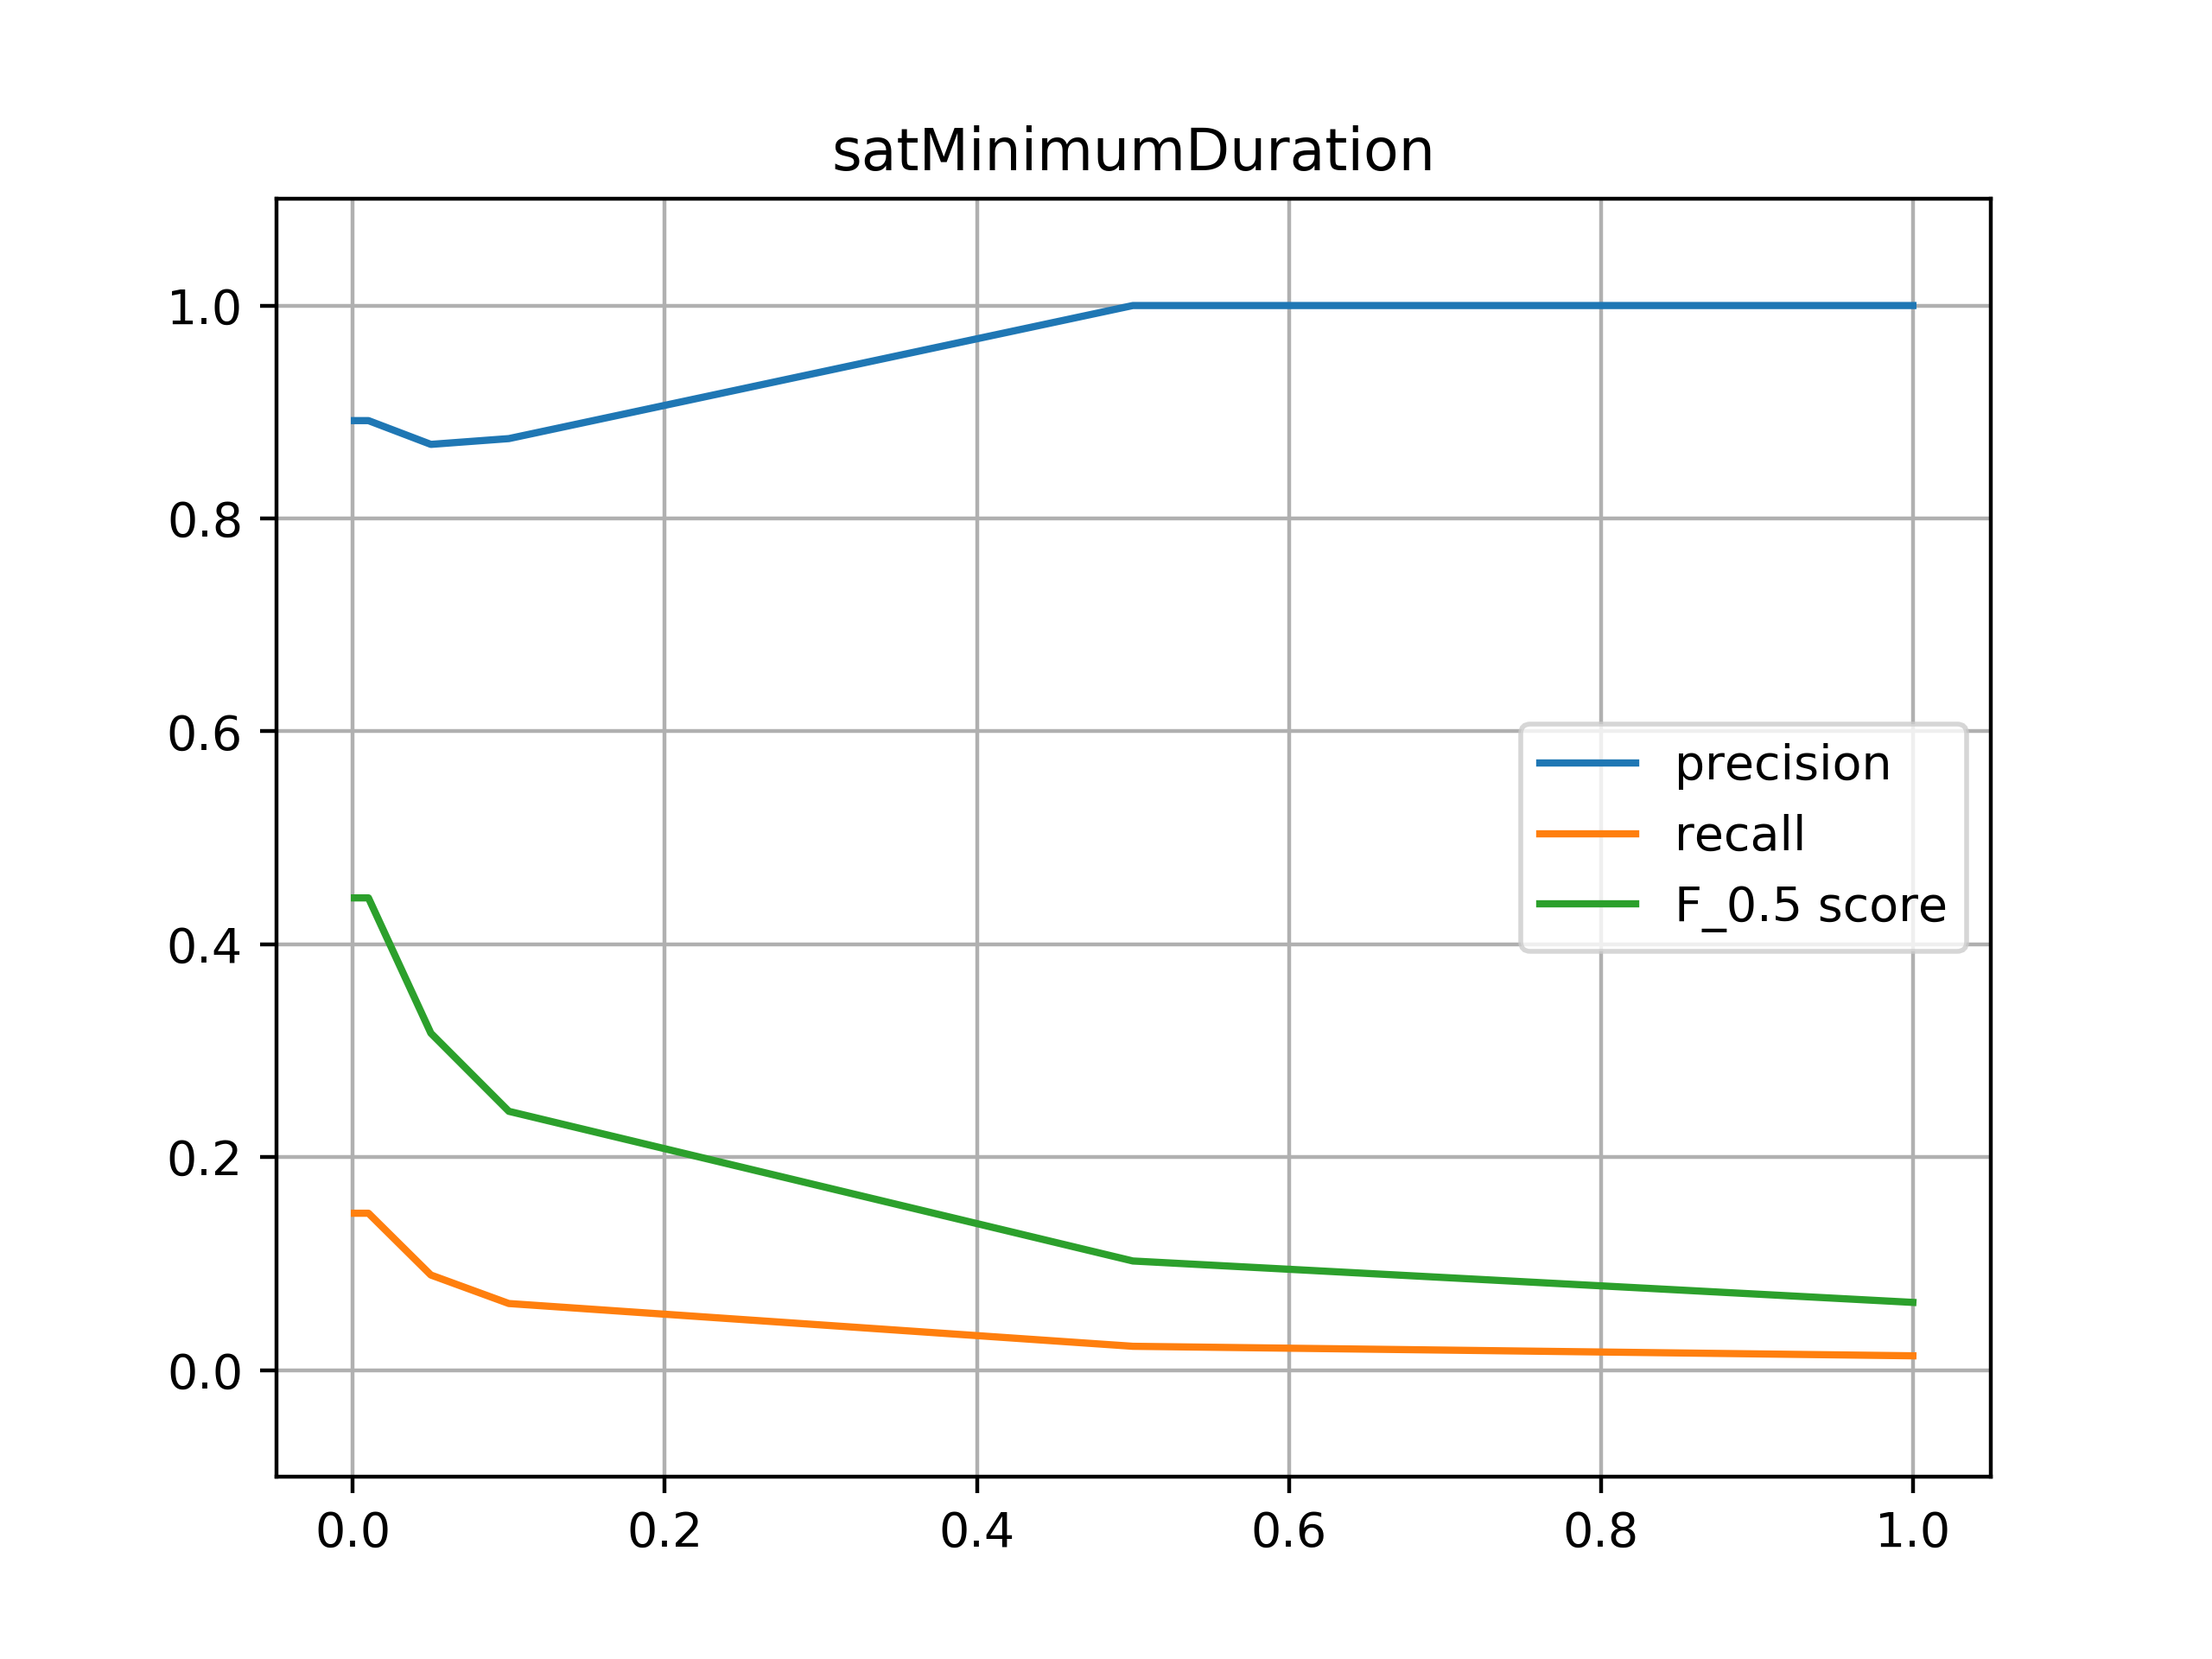
\includegraphics[clip,width=0.7\columnwidth]{Figures/satMinimumDuration.png}% 
	\caption{minimumDuration parameter sweep results (accuracy, F score and recall)}
	\label{fig:satMinimumDuration}
\end{figure}

\section{Silence detection evaluation}
For the silence detection algorithm, two parameters were evaluated: frameSize and threshold which for both we had simiar results as they were obtained in hum detection meaning that no audios were detected as having an issue.

\begin{figure}[H]
	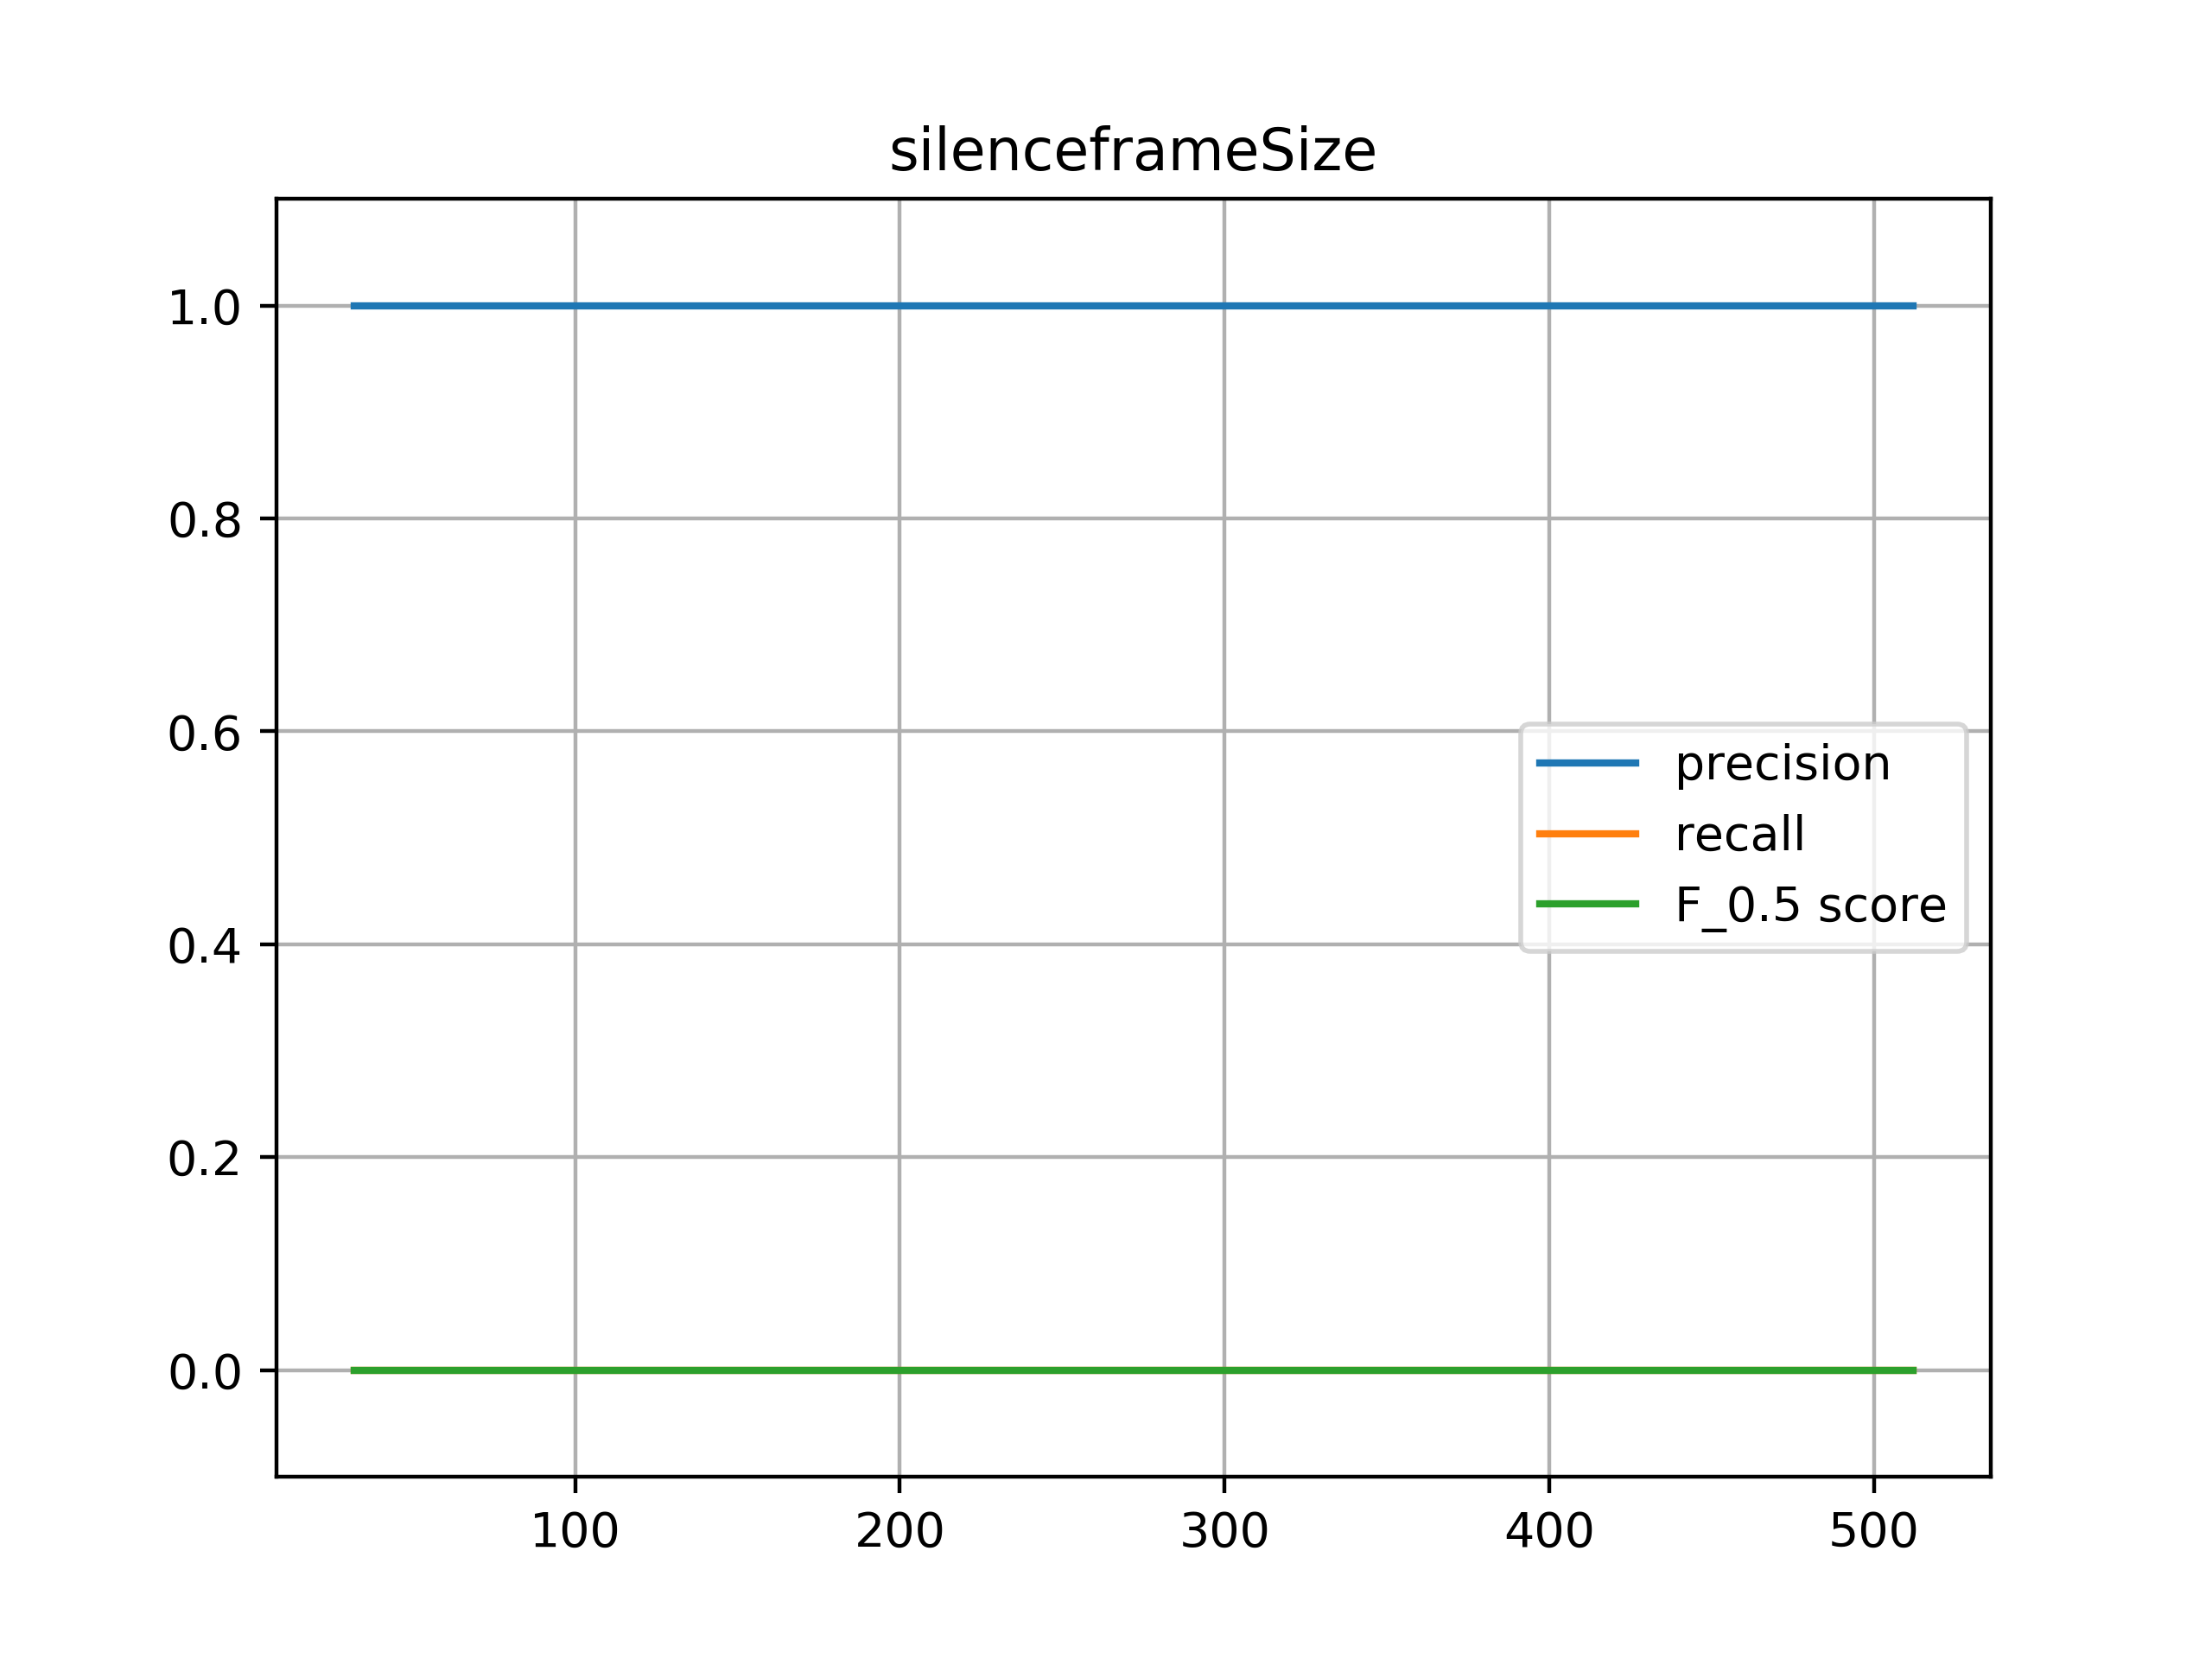
\includegraphics[clip,width=0.7\columnwidth]{Figures/silenceframeSize.png}% 
	\caption{frameSize parameter sweep results (accuracy, F score and recall)}
	\label{fig:silenceframeSize}
\end{figure}

\begin{figure}[H]
	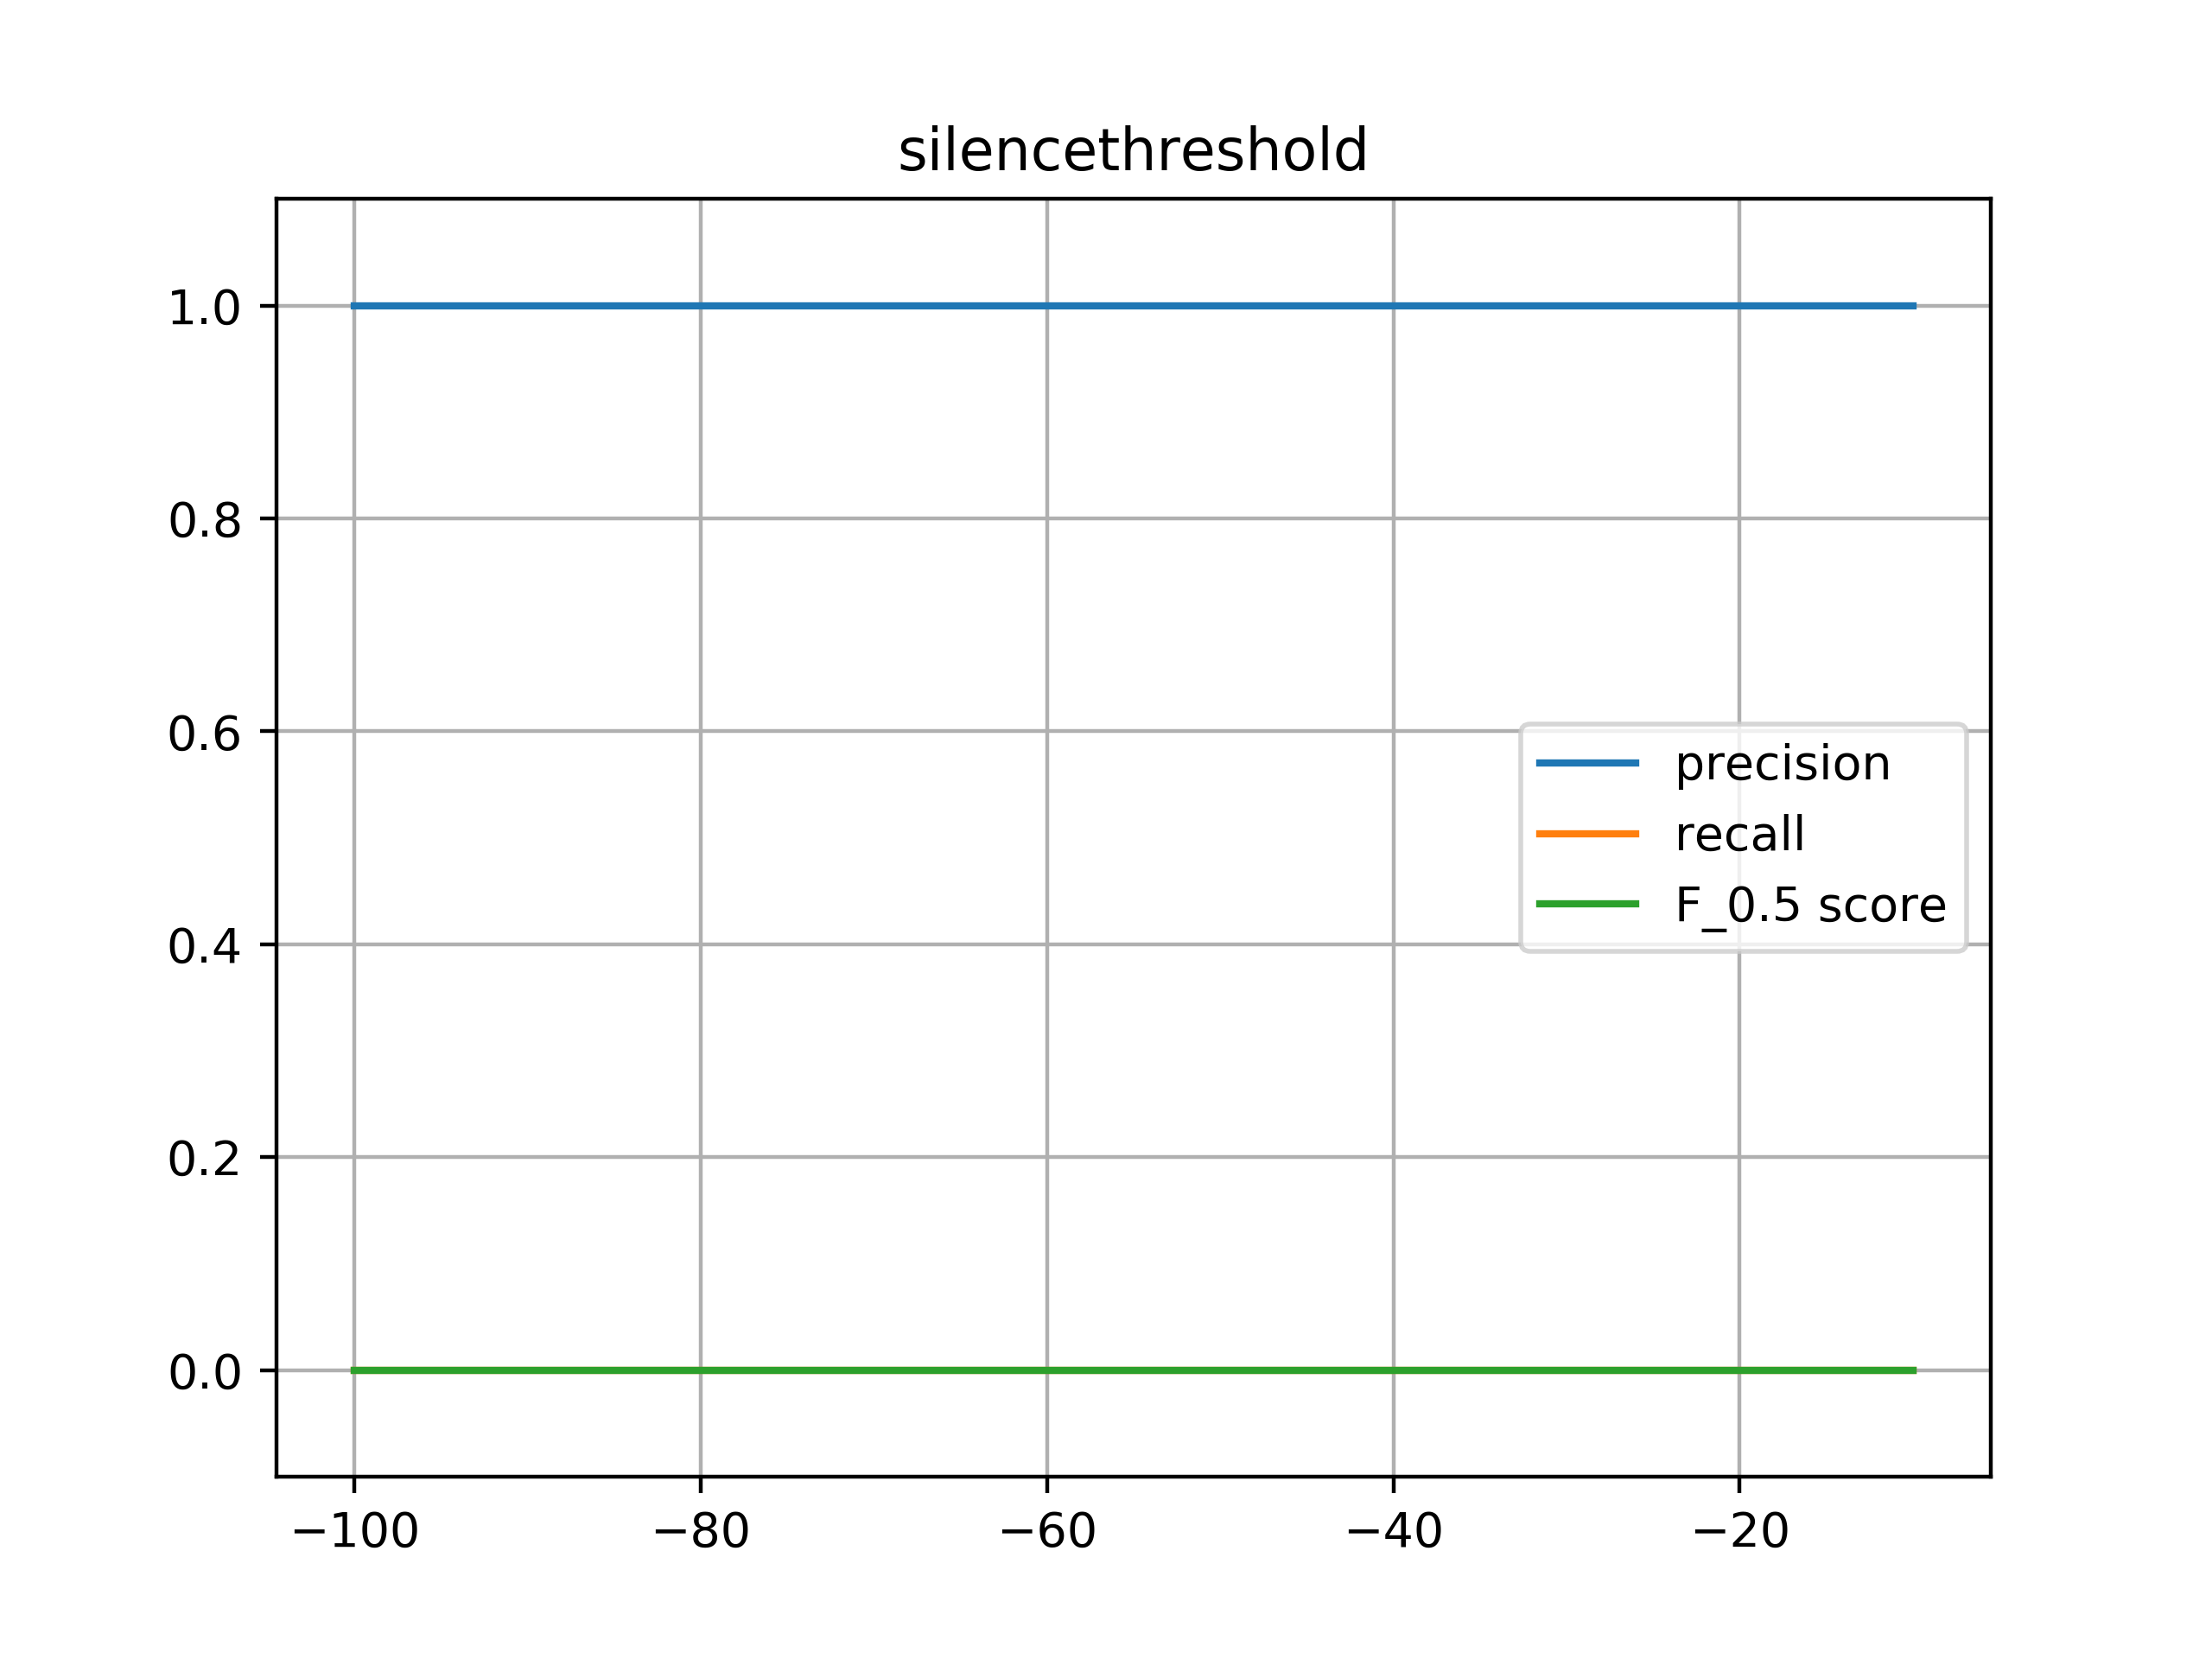
\includegraphics[clip,width=0.7\columnwidth]{Figures/silencethreshold.png}% 
	\caption{threshold parameter sweep results (accuracy, F score and recall)}
	\label{fig:silencethreshold}
\end{figure}

\newpage


